% !TeX spellcheck = it_IT
\section{Comunicazione Wireless}
Tutte le comunicazioni nel mondo wired avvengono tipicamente in banda base, i.e., data una banda $B$ trasmetto direttamente usando lo spettro di frequenze $[0,B]$.\\ 

Problemi:
\begin{enumerate}
	\item Se tutti i dispositivi trasmettessero in banda base, tutte le comunicazioni radio farebbero interferenza l'una con l'altra
	\item Più è bassa la frequenza più grande deve essere l'antenna ($\lambda/2$ per antenna dipole, es: $1MHz \sim 142$ metri, $2100MHz \sim 7$ cm)
	\item Ogni range di radio frequenze possiede diverse proprietà i propagazione e attenuazione
\end{enumerate}

\paragraph{Spettro elettromagnetico per le telecomunicazioni:}
\begin{center}
	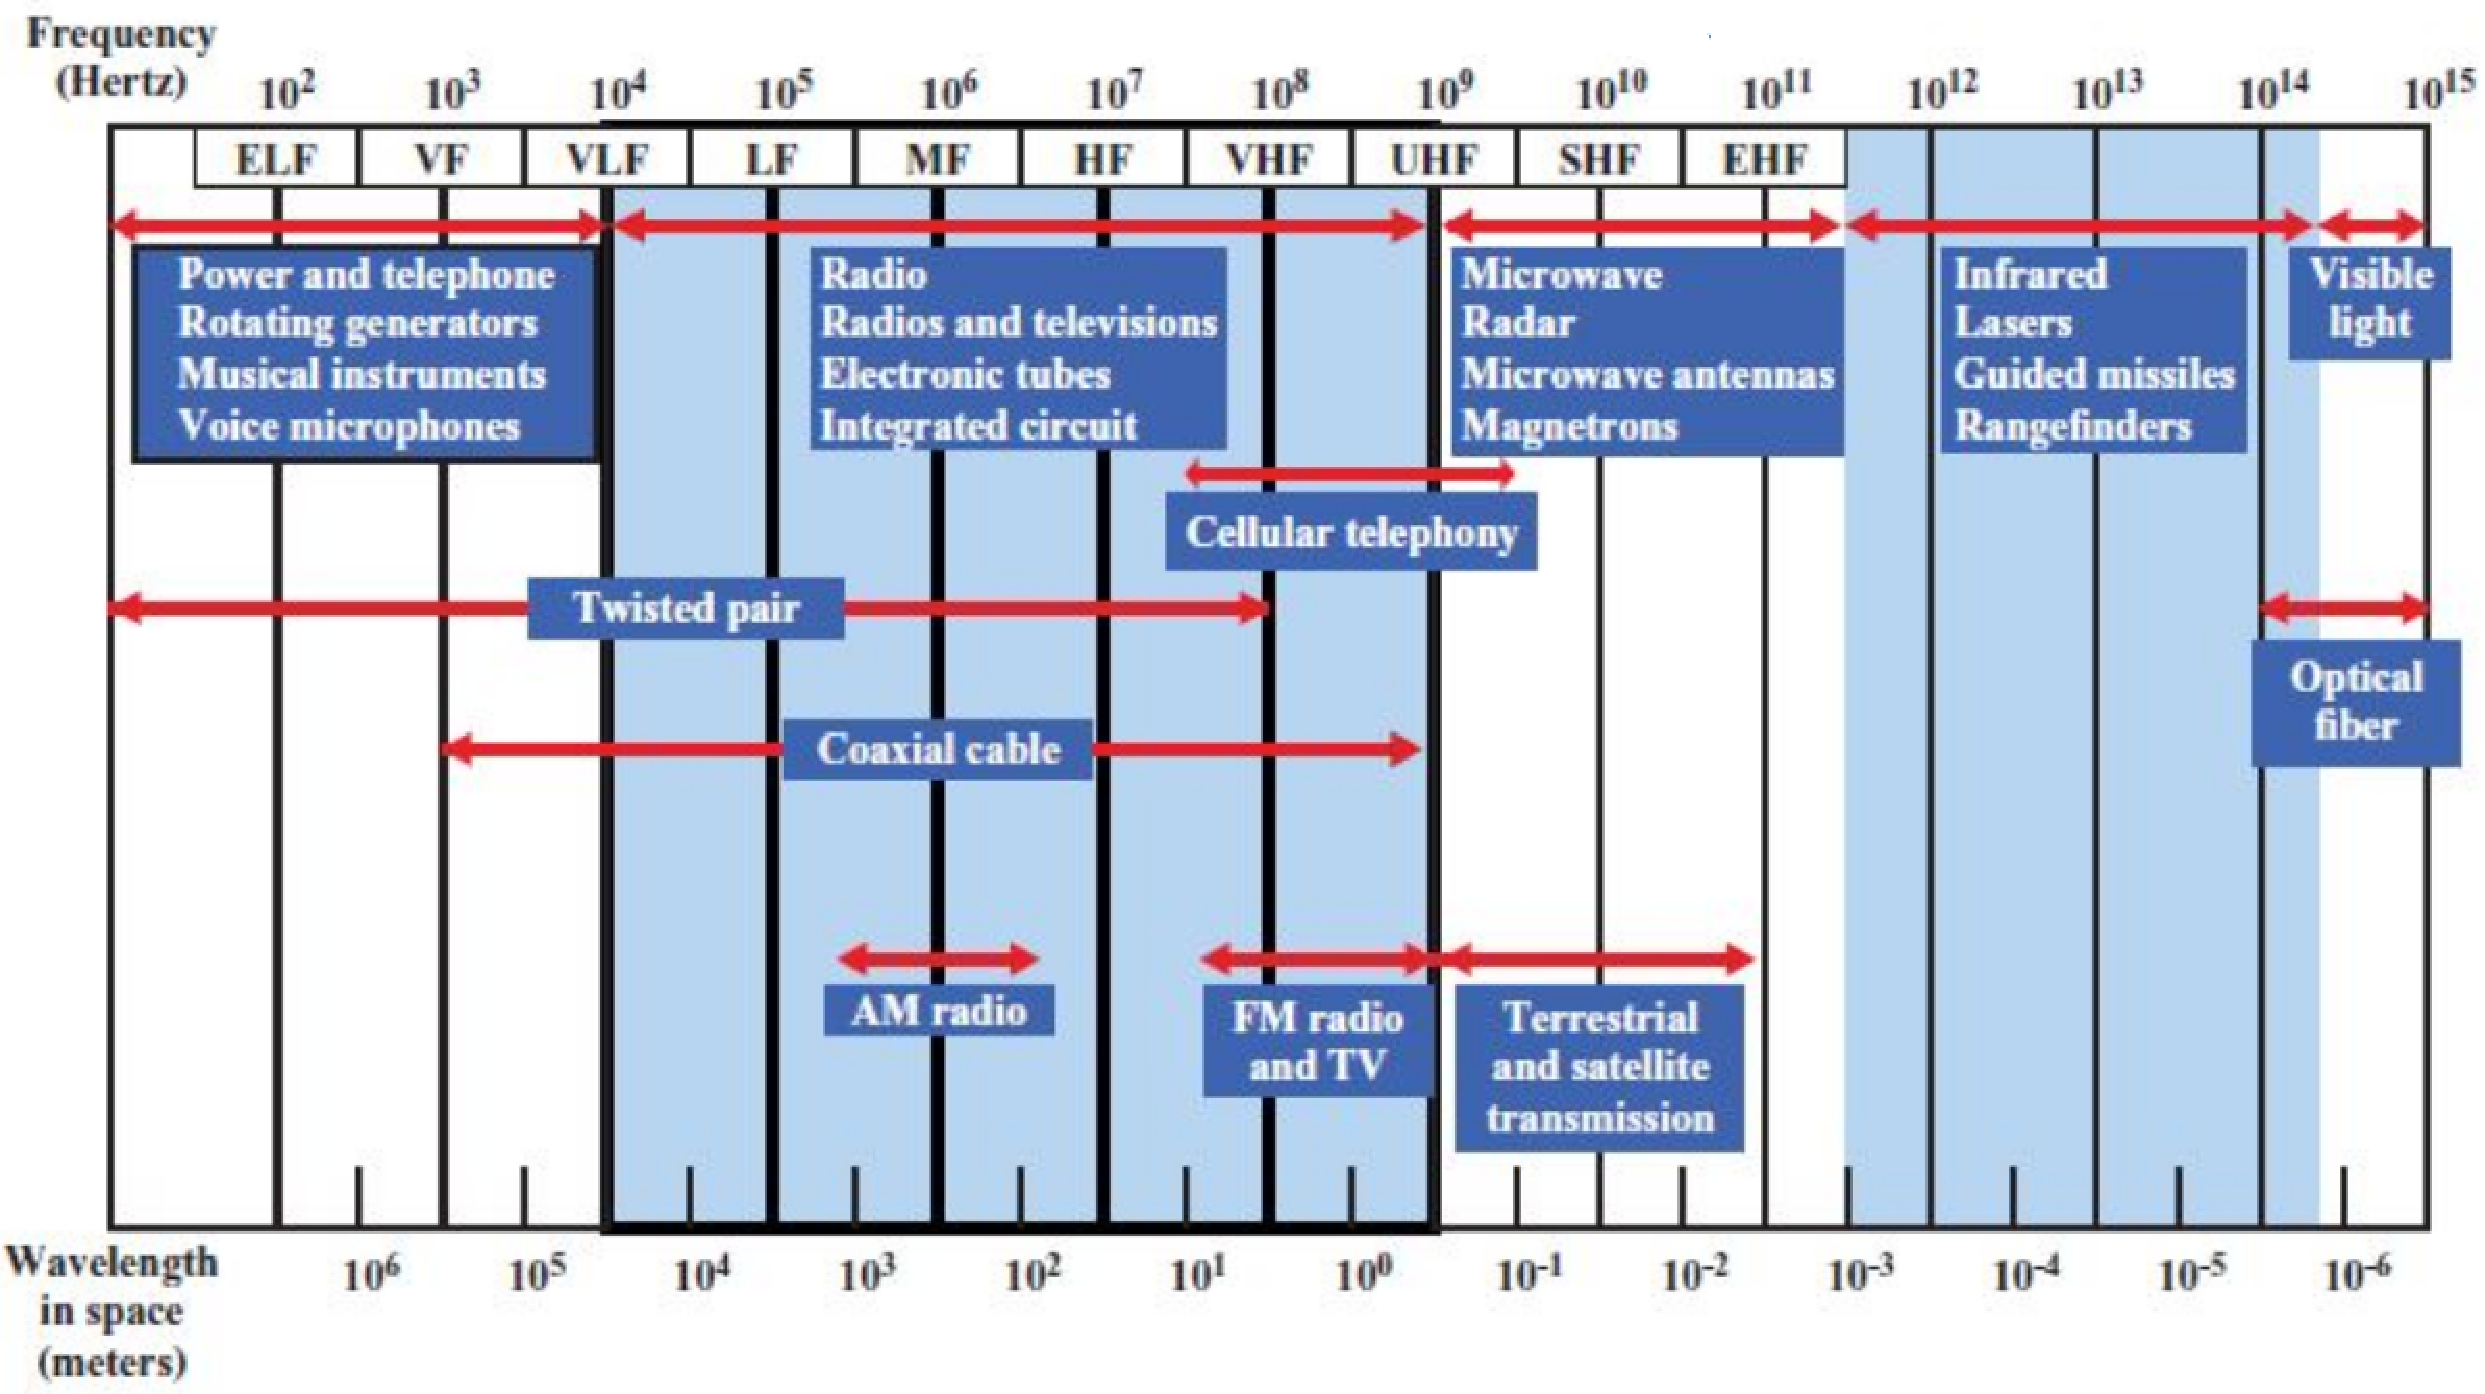
\includegraphics[width=0.98\linewidth]{img/wireless/emspectrum1}
\end{center}
Molto approssimativo, c'è uno standard per ogni tipo di telecomunicazione (\href{https://upload.wikimedia.org/wikipedia/commons/thumb/c/c7/United_States_Frequency_Allocations_Chart_2016_-_The_Radio_Spectrum.pdf/page1-1200px-United_States_Frequency_Allocations_Chart_2016_-_The_Radio_Spectrum.pdf.jpg}{\texttt{allocazione delle frequenze per gli USA}}).\\

\newpage

\paragraph{Trasmissione in banda traslata:} Da $[0,B]$ spostiamo la banda all'interno di un altro range, ovvero $[f_c - B/2, f_c + B/2]$, la stessa banda ma traslata attorno ad una frequenza portante $f_c$.
\begin{center}
	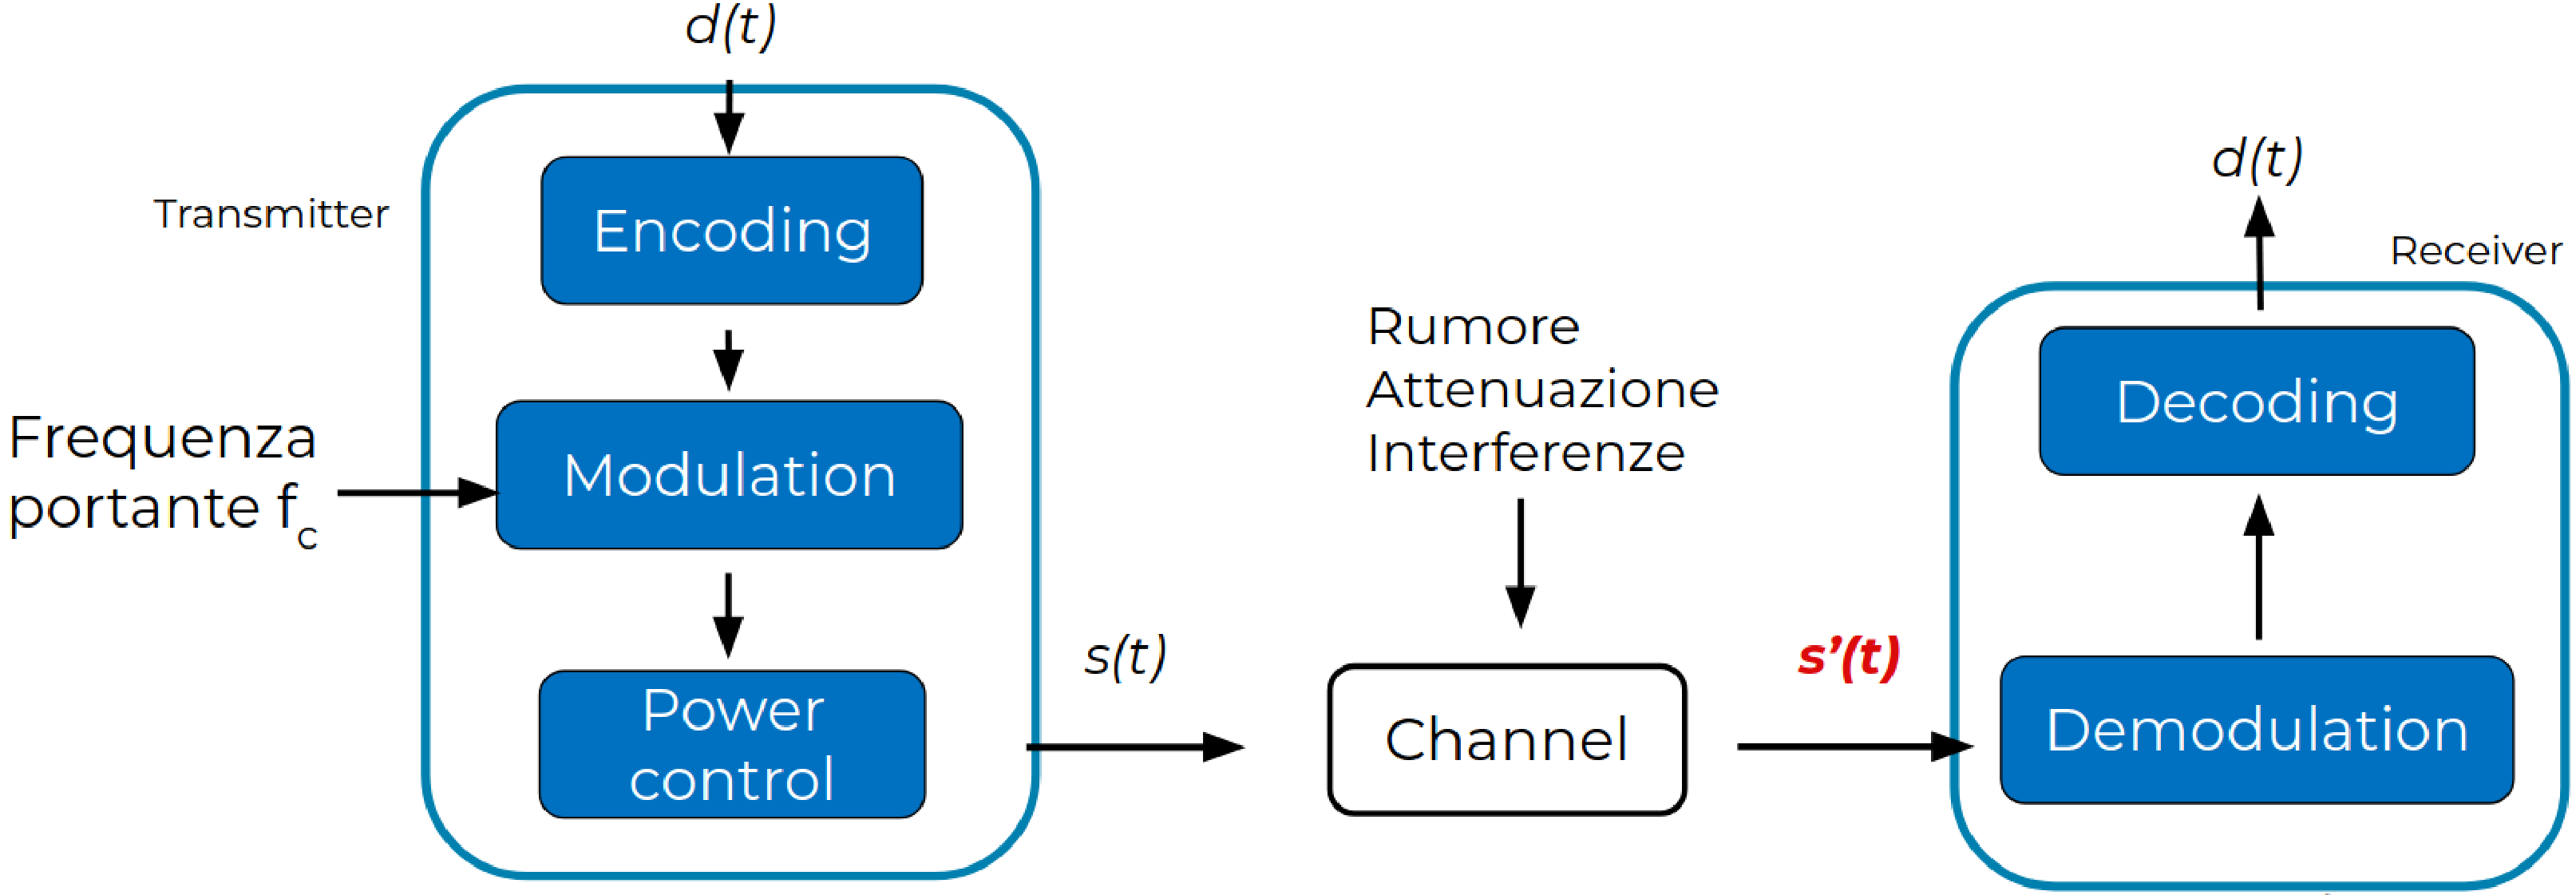
\includegraphics[width=0.95\linewidth]{img/wireless/bandatraslata1}
\end{center}
Il compito del trasmettitore diventa codificare, \textbf{modulare attorno alla frequenza portante} $f_c$ ed il trasmettitore deve de-modulare, pulire e decodificare il segnale trasmesso. Bandwidth e data rate rimangono gli stessi, cambia solo "dov'è" la banda.\\

Domande: 
\begin{enumerate}
	\item Che spettro utilizzare? (che frequenza portante scegliere)
	\item Come codifico i dati? (da digitale ad analogico)
	\item Come modulo il mio segnale in banda base sulla frequenza portante?
\end{enumerate}

\newpage

\subsection{Encoding, symbol e symbol rate}

\paragraph{Simbolo:} Una forma d'onda, uno stato o una condizione significativa del canale di comunicazione che persiste per un intervallo di tempo fissato. Esempio: voltaggio a $3V$ per 1 secondo.\\

\paragraph{Symbol rate:} Quantità di simboli trasmessi al secondo (misurato in baud). Dipende dal processore fisico.\\

In generale, un \textbf{simbolo può contenere più bit} (codifica e modulazione), quindi \textbf{symbol rate $\neq$ bit rate}.\\
Generalmente, più la distanza da coprire si allunga più la durata si abbassa.\\

Una data bandwidth può supportare diversi data rate, a seconda dell'abilità del ricevente di distinguere 0 e 1 in presenza di rumore.\\

Possiamo codificare tramite una modulazione in ampiezza: data una entry di bit scegliamo il voltaggio corrispondente
\begin{center}
	\includegraphics[width=\linewidth]{img/wireless/modam1}
\end{center}
Moduliamo la portante (modifichiamo l'ampiezza) in base ai bit da codificare. Usato nelle radio AM. Si può vedere che symbol rate e data rate sono diversi, ogni simbolo (livello di ampiezza) rappresenta due bit.\\

\newpage

\subsection{Trasmissione delle onde radio}

\paragraph{Propagazione onde radio:} Ci sono più possibili tipi di propagazione delle onde radio, in base alla frequenza utilizzata
\begin{itemize}
	\item Ground Wave Propagation (sotto i $2MHz$): il segnale segue la curvatura della terra
	\item Sky Wave Propagation (da $2$ a $30MHz$): il segnale rimbalza nella ionosfera
	\item \textbf{Line of Sight LoS} (sopra $30MHz$): Deve esserci una linea diretta (anche non a vista in realtà, ma diretta) tra trasmettitore e ricevitore
\end{itemize}

\paragraph{Tipi di antenne:}
\begin{itemize}
	\item Omnidirezionale (a sinistra), la potenza emessa è uguale in tutte le direzioni (ideale)
	\item Direzionale (a destra): si vuole propagare segnale in una sola direzione, non ideale, ma solitamente la propagazione non è limitata strettamente ad una direzione
\end{itemize}
\begin{center}
	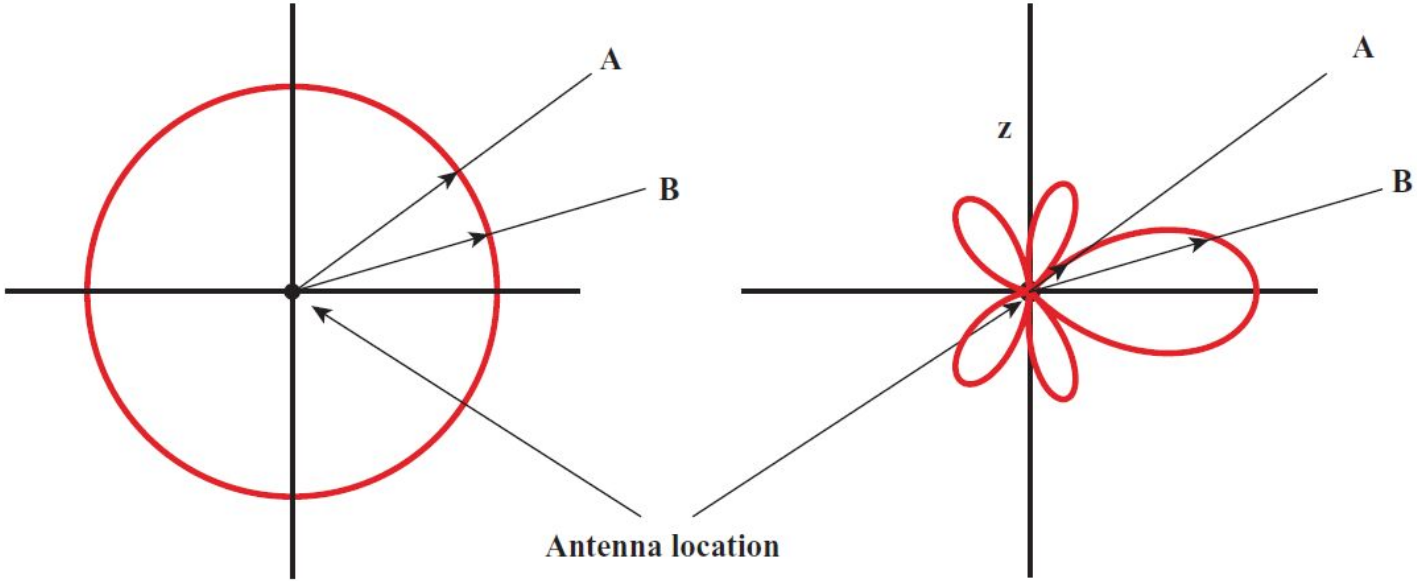
\includegraphics[width=0.9\linewidth]{img/wireless/antenna}
\end{center}

\newpage

\subsubsection{Problemi con Trasmissione radio Line of Sight (LoS)}

Ci sono problemi legati alla trasmissione LoS:
\begin{itemize}
	\item Free space loss \& path loss: attenuazione del segnale dovuta alla distanza e all'ambiente in cui il segnale si propaga; cosa perdo da antenna trasmettitrice (TX) a ricevitrice (RX)
	\item Rumore: disturbo che può distorcere il segnale
	\item Multipath: il segnale tra TX e RX può subire riflessioni, diffrazioni e scattering causando la ricezione di più onde elettromagnetiche dello stesso segnale in tempi diversi; per qualche motivo, un riflesso del segnale giunge al ricevitore, in momenti diversi dall'originale, possono diventare interferenze per segnali successivi
	\item Effetto Doppler: Il segnale cambia a causa del movimento di RT, TX e ostacoli; il segnale ricevuto potrebbe essere su una frequenza "vicina" a quella originale, disturbando la fingerprint di un segnale
\end{itemize}

\paragraph{Path Loss:} Attenuazione del segnale radio in funzione della distanza tra trasmettitore e ricevitore.
$$ \frac{P_t}{P_r} = \left(\frac{4 \pi}{\lambda}\right)^2 d^n = \left(\frac{4 \pi f}{c}\right)^2 d^n $$
Misurata in $dB$, rapporto tra potenza del segnale trasmesso (fisso) rispetto alla potenza del segnale ricevuto (diventa sempre più piccolo, in base alla distanza).\\

Direttamente proporzionale (al quadrato della) alla frequenza, direttamente proporzionale ad una potenza della distanza, l'esponente $n$ dipende dall'ambiente (più l'ambiente è ostruito più la distanza sarà influente).\\

%End L2

\newpage

%Start from s54
\paragraph{Free space loss ($n=2$):} A parità di distanza, maggiore è la frequenza maggiore è il path loss. La potenza di trasmissione massima è regolamentata (standard). A parità di potenza, maggiore è la frequenza minore è il raggio di copertura. Con "free space loss" si intende la perdita ideale in caso di spazio completamente libero, quindi con $d^n = d^2$.
\begin{center}
	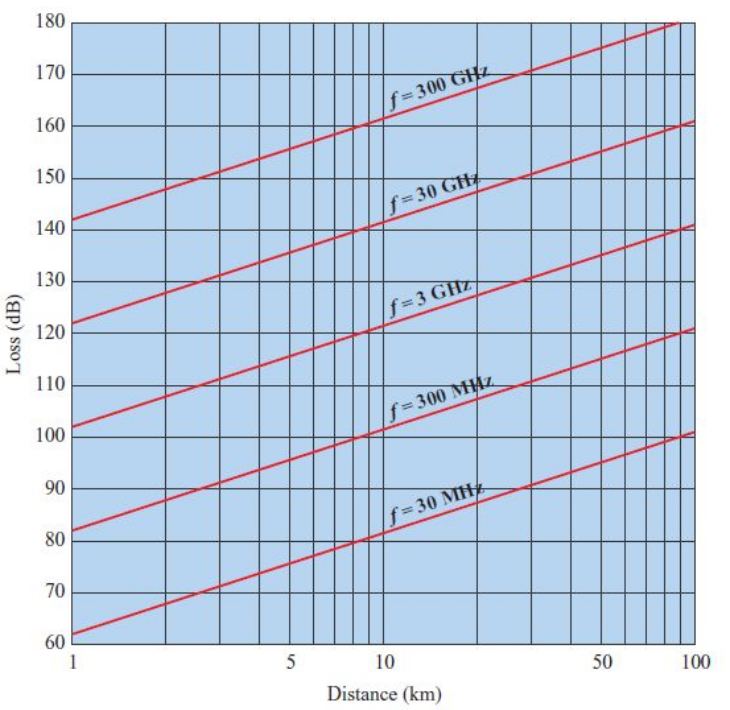
\includegraphics[width=0.75\linewidth]{img/wireless/freespaceloss}
\end{center}

Con $300GHz$ la perdita ad 1km è oltre i $140db$, mentre con $30MHz$ è poco sopra i $60dB$. La distanza di trasmissione è limitata dalle frequenze utilizzate da una certa tecnologia.\\

\newpage

\paragraph{Antenna gain:} La diffusione di un'antenna ideale è isotropica (in tutte le direzioni), ma questo può essere inefficiente, capendo la posizione dei ricevitori si può migliorare la potenza ricevuta. L'idea di un'antenna direzionale è convogliare l'energia verso un determinato punto, un "beam" verso il ricevitore. Il segnale si propaga in una ellisse verso la direzione voluta dall'antenna, al contrario del cerchio creato da un'antenna isotropica.\\

Il \textbf{gain} di un'antenna viene definito come il rapporto tra l'intensità della radiazione elettromagnetica in una data direzione e l'intensità che si avrebbe se si usasse un'antenna isotropica, misurato in $dBi$. La direzionalità viene misurata in $dBi$, dove $i$ sta per "isotropic", ed è il rapporto tra la potenza che si avrebbe in quel punto con una antenna isotropica al denominatore e l'antenna attuale al numeratore. Concentrando verso il ricevitore "perdo" verso le altre direzioni. \\

%Le formule sono sempre quelle dei dB
Questo ha un \textbf{effetto sul path loss}; nel caso ideale avremmo allineamento perfetto tra TX e RX e di conseguenza un gain che riduce la perdita di potenza nella trasmissione. \\

Alla perdita in free space, si sottraggono valori dipendenti dal gain di trasmittente e ricevente, abbassando il rapporto e riducendo la perdita. Chiamando $G_{tx}$ e $G_{rx}$ gain di trasmettitore e ricevitore, rispettivamente: 
$$ \frac{P_t}{P_r} = \frac{(4 \pi f)^2}{G_{tx} G_{rx} c^2} d^n $$
Da ricordare che è necessaria un allineamento, se il ricevitore è fuori dal "beam" allora la potenza ricevuta sarà minore di quella di un antenna isotropica, a parità di distanza ($dBi$ negativi, il gain peggiora).\\

\newpage

\paragraph{Multipath:} Anche se direzionale, il segnale avrà una "fascia" di direzioni in cui viene inviato, quindi può interagire con l'ambiente: 
\begin{itemize}
	\item \textbf{riflessione:} il segnale "rimbalza", come su uno specchio, 
	\item \textbf{scattering:} quando la lunghezza d'onda $\lambda$ è simile a quella dell'oggetto, un raggio colpisce l'elemento e viene separato in tanti altri, sparsi in tutte le direzioni 
	\item \textbf{diffrazione:} se la lunghezza d'onda è $\lambda \ll$ della dimensione di un oggetto e lo colpisce sui bordi, diffondendo il segnale in più direzioni dall'altro lato dell'oggetto
\end{itemize}
\begin{center}
	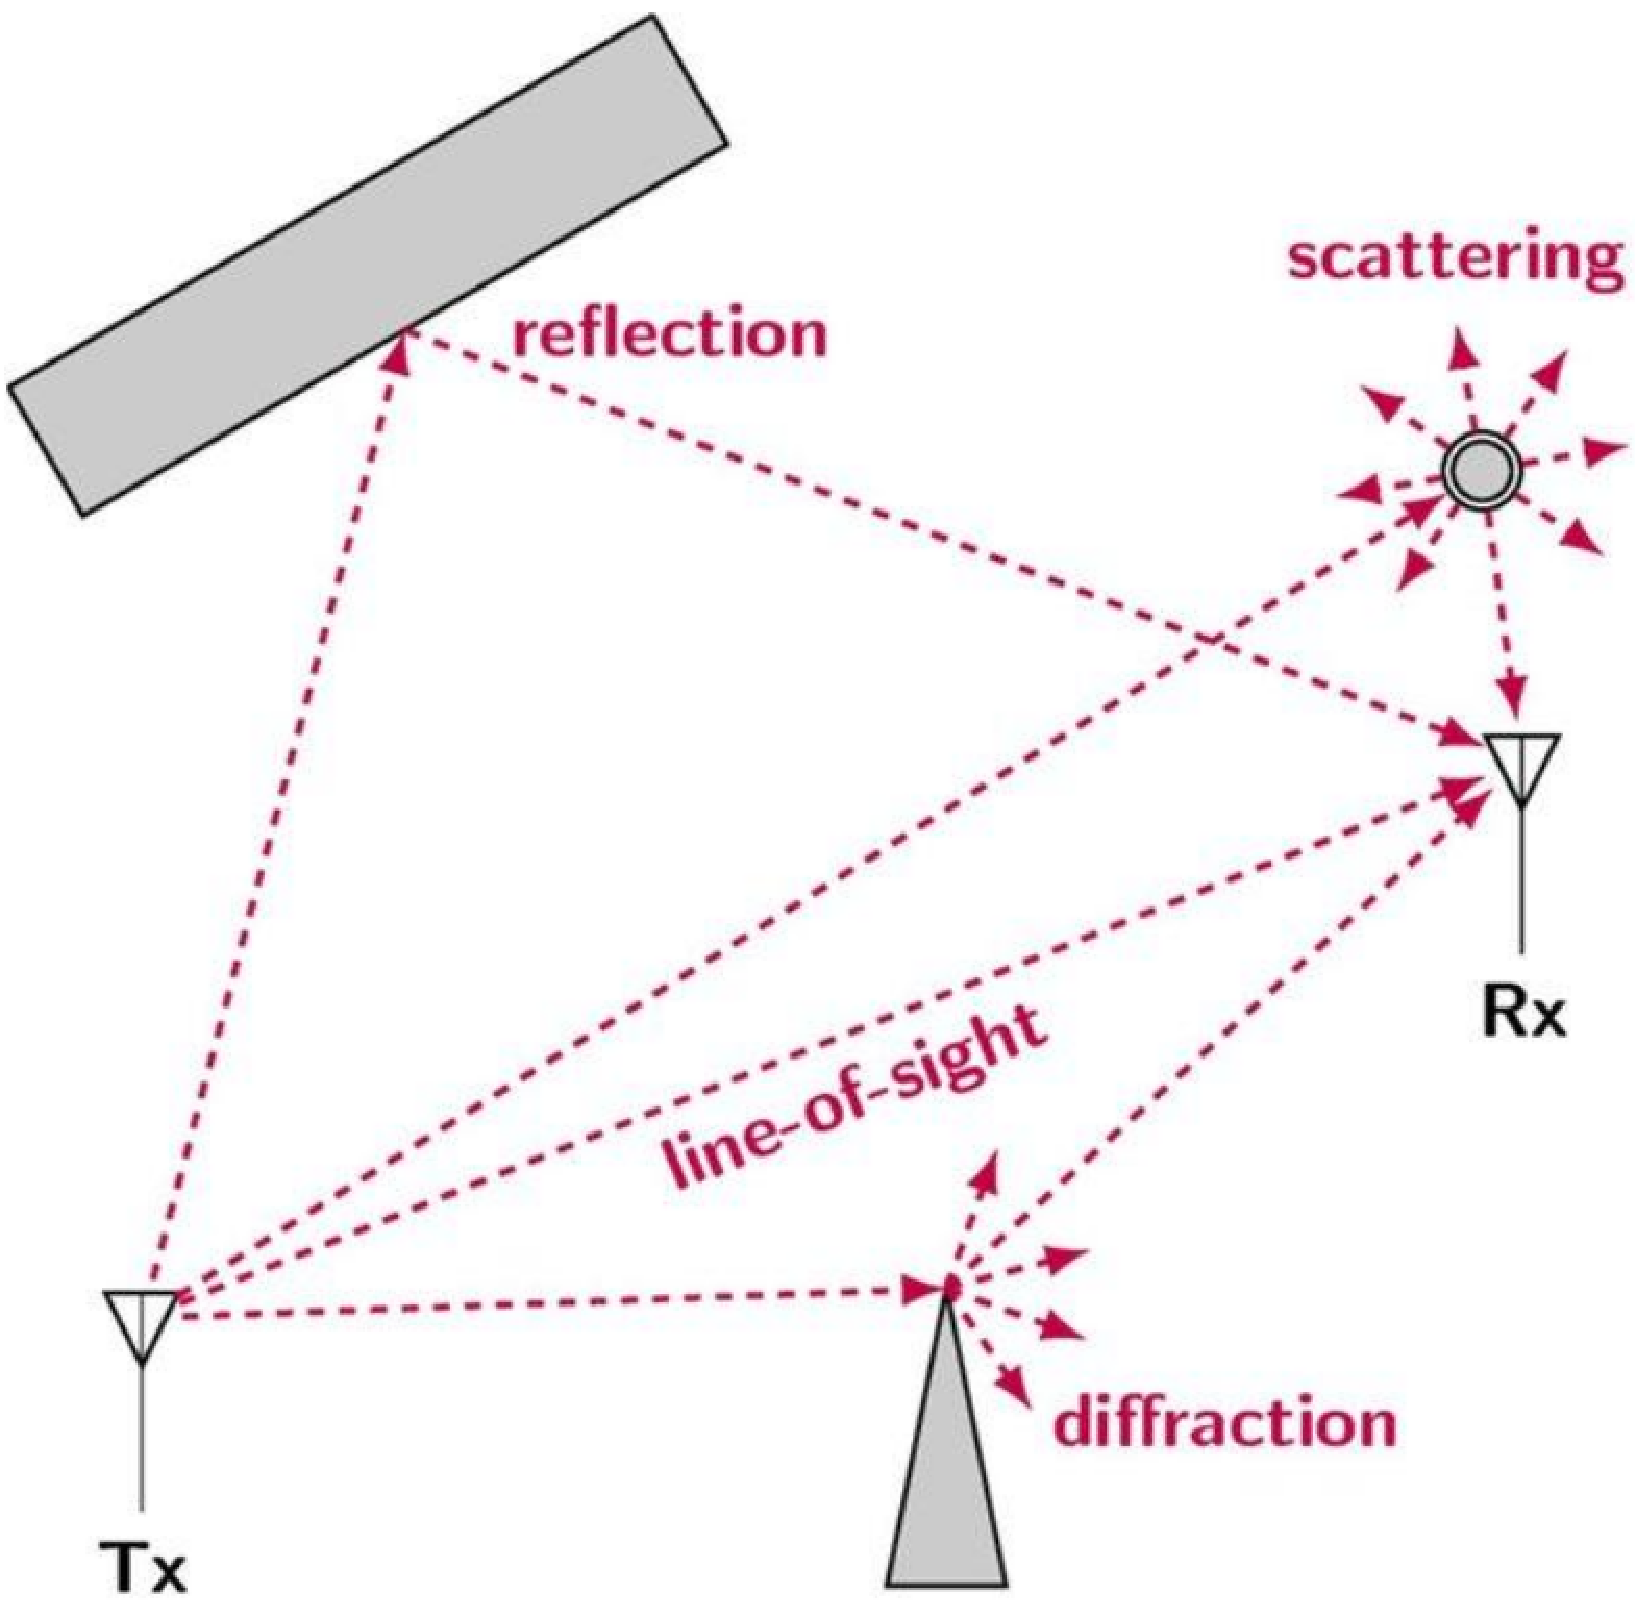
\includegraphics[width=0.7\linewidth]{img/wireless/multipath1}
\end{center}
I percorsi che non sono LoS saranno più lunghi e, di conseguenza, più lenti.  \\

\newpage

\paragraph{Fading:} Quando più segnali vengono ricevuti in tempi diversi ci sono due tipi di interferenze: 
\begin{itemize}
	\item \textbf{costruttiva:} "fa bene", aumenta l'ampiezza ed il segnale
	\item \textbf{distruttiva:} il segnale ricevuto viene modificato in modo imprevedibile (fading/evanescenza)
\end{itemize}
\begin{center}
	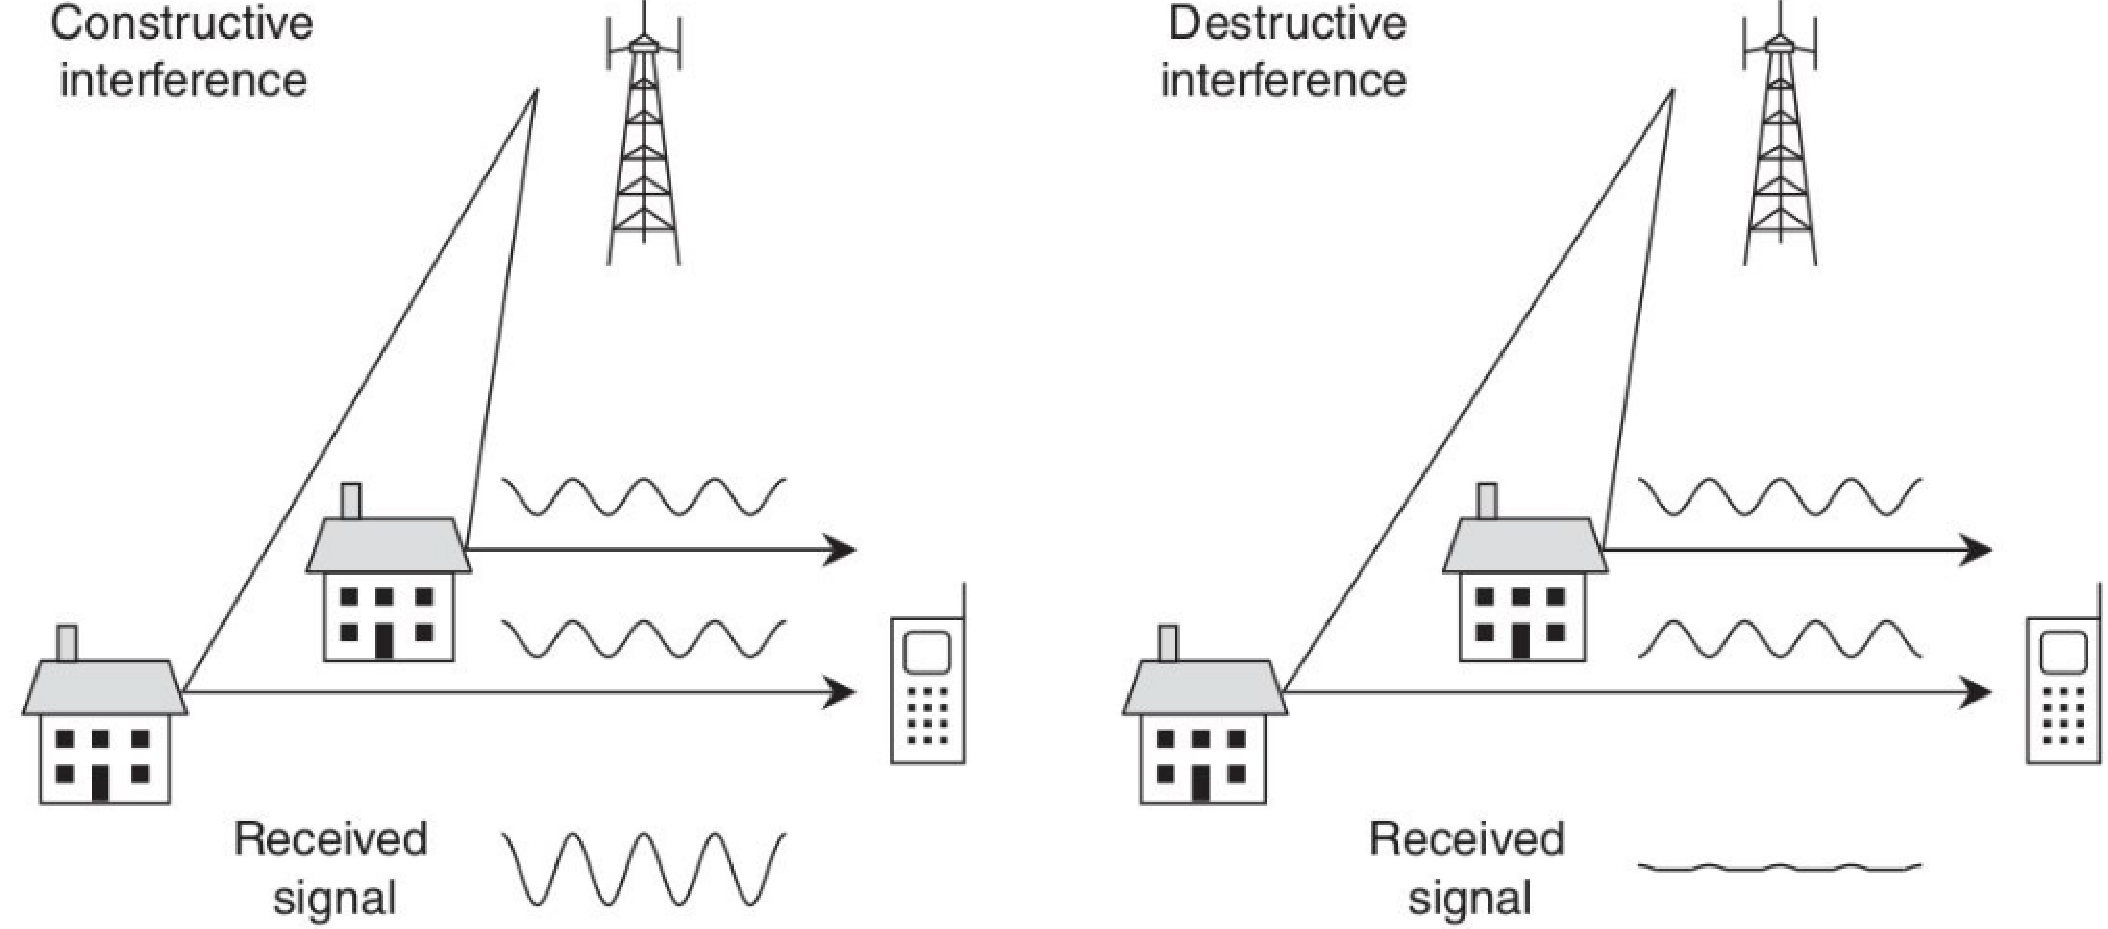
\includegraphics[width=0.85\linewidth]{img/wireless/fading}
\end{center}

Bisogna tenere conto delle proprietà fisiche del mezzo, quindi da come il segnale si modifica durante la propagazione. Il \textbf{Coherence time} permette di avere una stima per sapere ogni quanto campionare la condizione di un canale, un lasso di tempo in cui essere sicuri che il canale non subirà cambiamenti significativi; scala temporale in cui le caratteristiche del segnale sono "costanti"
$$ T_c = \frac{1}{f_D}$$

Dove $f_D$ è la \textbf{frequenza di Doppler}: dipende dalla velocità di movimento tra trasmettitore e ricevitore e dalla frequenza (e velocità della luce); più alta è la frequenza o più velocemente ci muoviamo più il campionamento dovrà essere fitto
$$ f_D = \frac{v}{c} f_c$$

Una tecnologia pensata per determinati spettri ed una determinata velocità relativa possiamo determinare una stima di $T_c$ e costruire apparati che funzionano di conseguenza.\\

\newpage

Esempio:
\begin{center}
	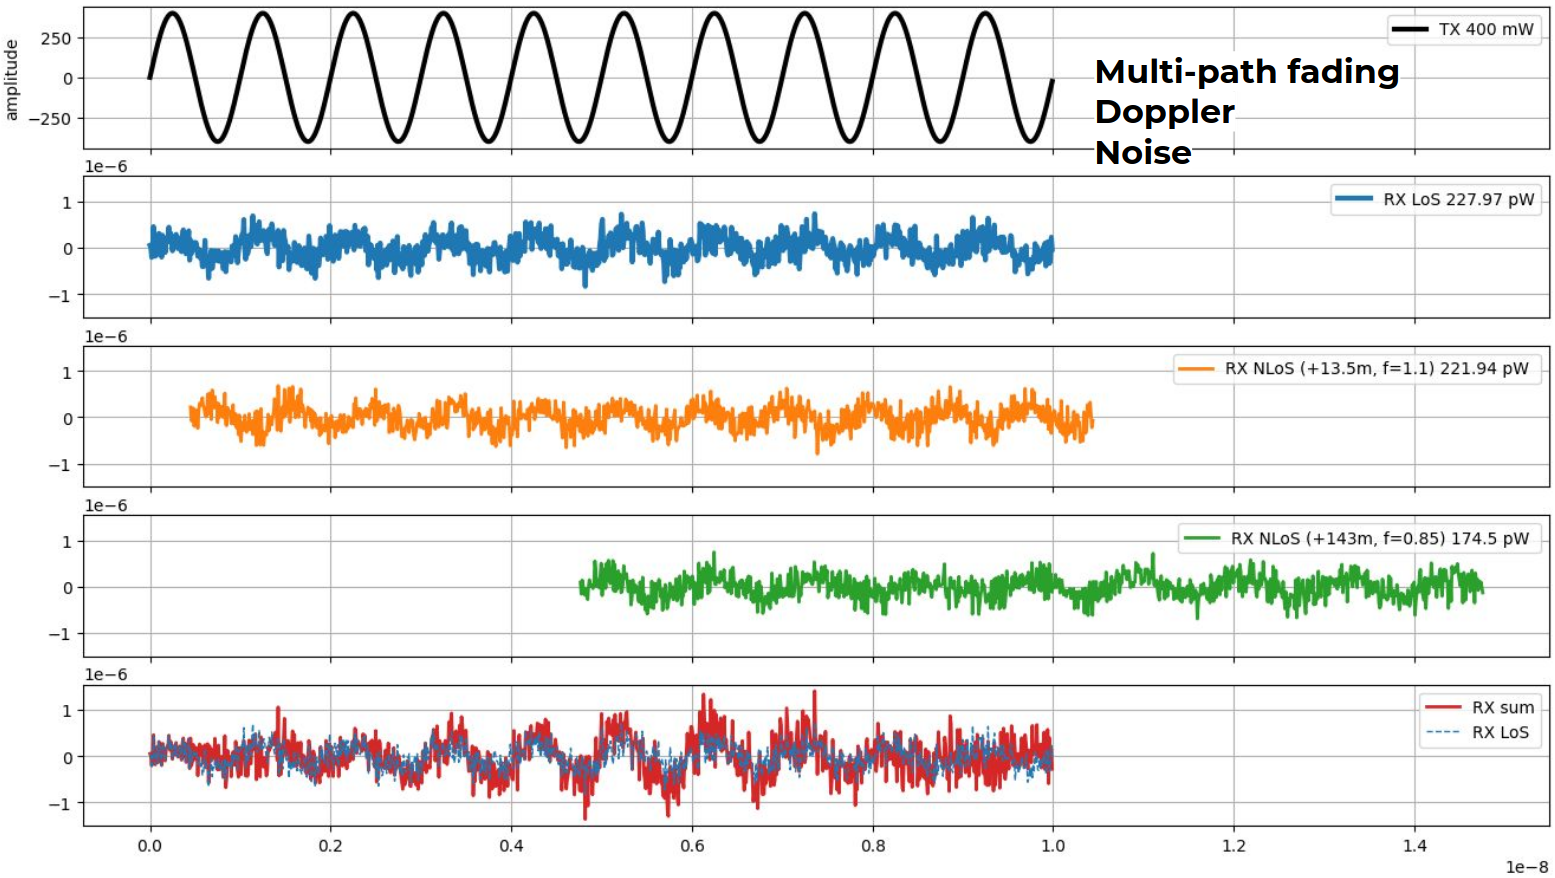
\includegraphics[width=0.9\linewidth]{img/wireless/examplemultipath}
\end{center}
I primi 4 grafici sono:
\begin{itemize}
	\item segnale trasmesso
	\item segnale ricevuto LoS, in $pW$, con effetto Doppler e noise
	\item altri 2 segnali NLoS (Non Line of Sight), percorrono più spazio, vengono ricevute dopo nel tempo e con una potenza ridotta, oltre che subire effetto Doppler e noise
\end{itemize}
L'ultima è ciò che viene effettivamente ricevuto, ovvero la combinazione di tutte le onde ricevute. E questo solo con il multipath, bisogna aggiungere anche effetto doppler e noise. \\

\newpage

\paragraph{Inter-Symbol Interference:} La lunghezza dei vari simboli deve tenere conto degli effetti del multipath. 
\begin{center}
	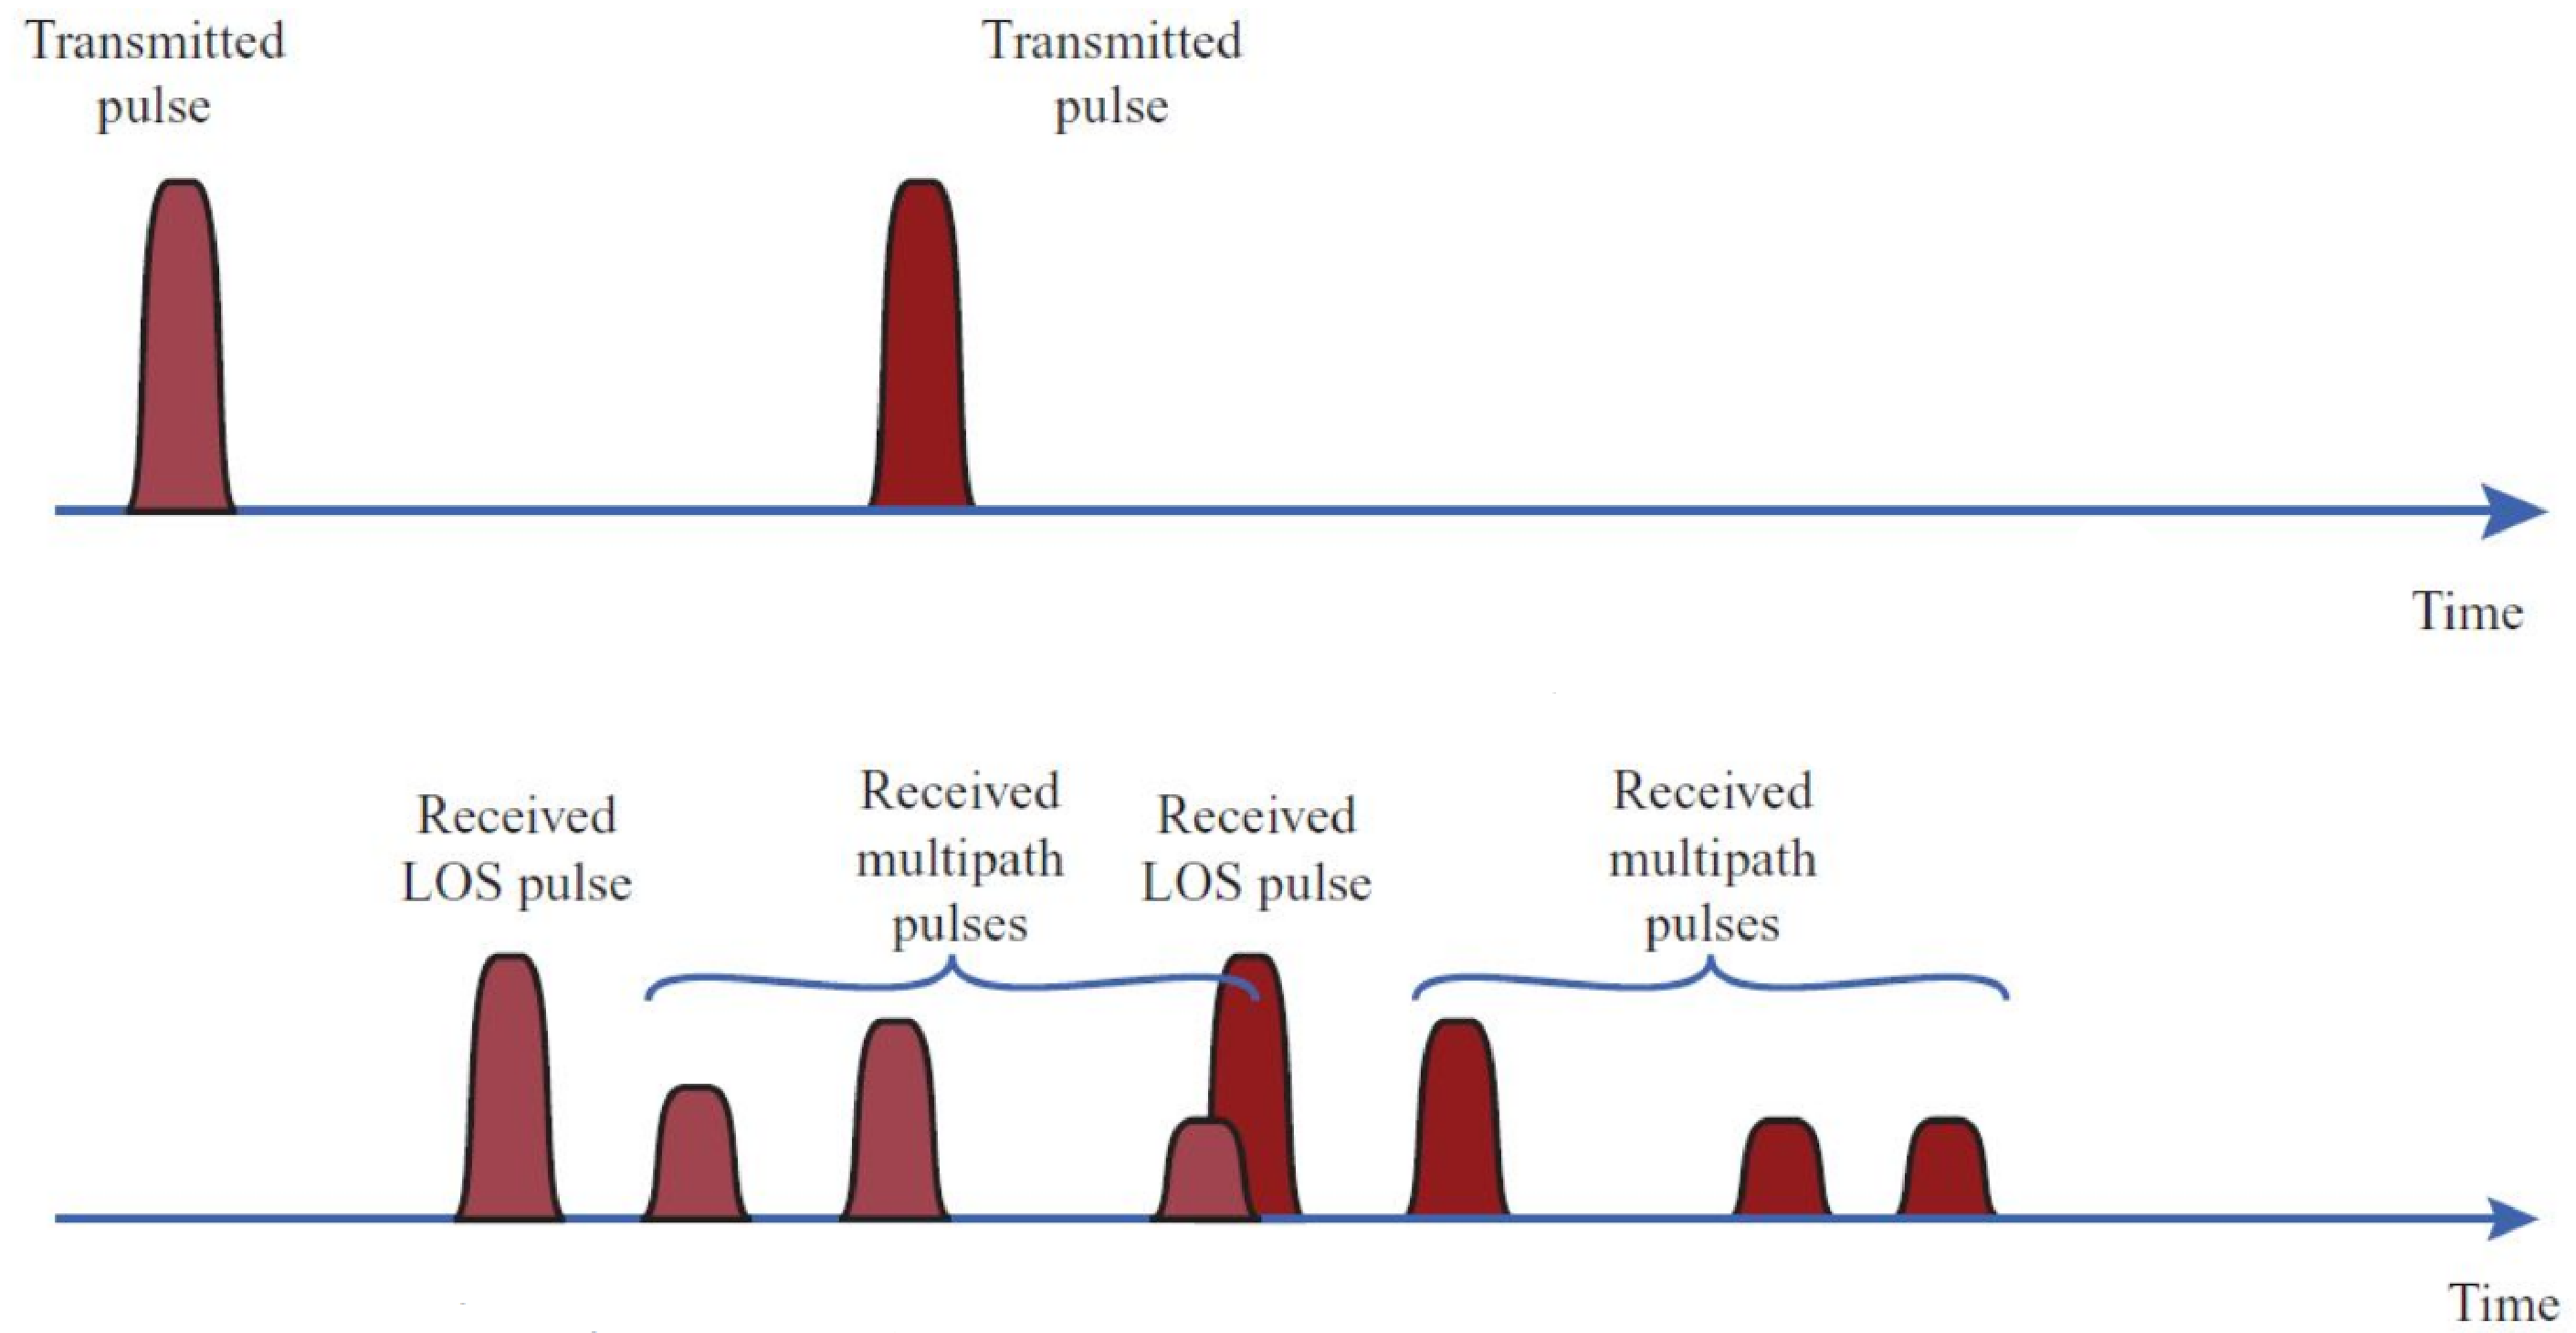
\includegraphics[width=0.8\linewidth]{img/wireless/ISI1}
\end{center}
Dopo il primo impulso LoS, vengono ricevuti altri simboli per effetto del multipath e ci possono essere altri segnali che interferiscono con l'impulso LoS successivo. Si sovrappongono segnali LoS e multipath di quello precedente, causando interferenza distruttiva, interferenza inter-simbolo ISI. La distanza tra un segnale e l'altro è troppo breve.\\

Maggiore è la distanza tra TX e RX, più alta è la probabilità di questi fenomeni. Trasmettendo meno simboli ho un data rate minore, ma incrementandoli aumenta la probabilità di avere ISI. \\

\newpage

\subsection{Codifica e Trasmissione Dati}
La struttura di una trasmissione radio è
\begin{center}
	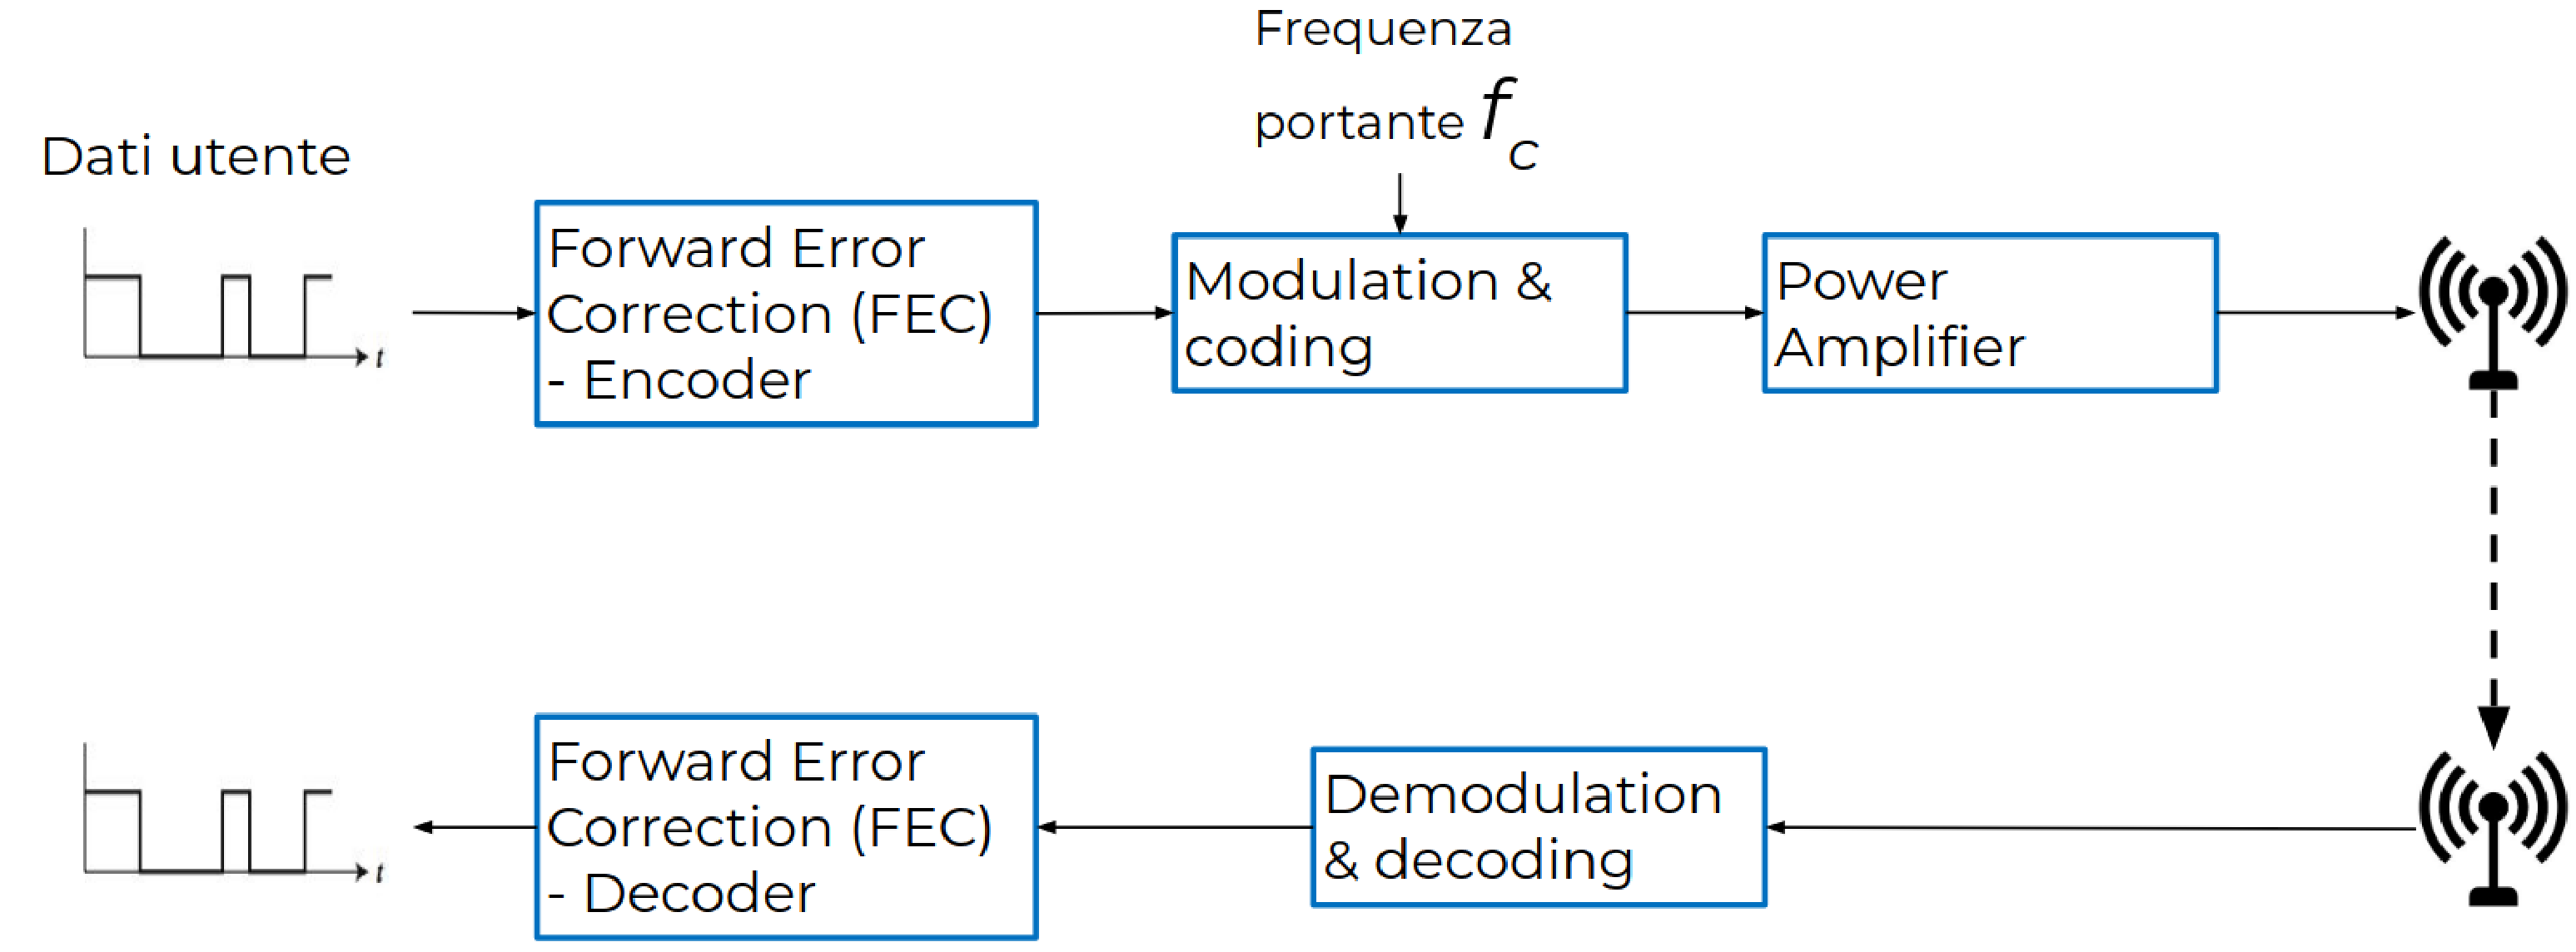
\includegraphics[width=0.95\linewidth]{img/wireless/struttrasmissione}
\end{center}

Le fasi sono: 
\begin{itemize}
	\item Forward Error Correction FEC
	\item Modulazione e encoding
	\item Si amplifica la potenza in modo da renderla sufficiente (secondo il path loss previsto), deve essere in grado di raggiungere il RX
	\item il segnale "brutto" ricevuto va demodulato e decodificato
	\item FEC sul decoder
\end{itemize}

\subsubsection{Modulazione e Codifica}
Per la codifica possiamo agire sui 3 parametri di una sinusoidale:
\begin{itemize}
	\item \textbf{Amplitude Shift Keying ASK:} diversi livelli di ampiezza per diversi bit
	\item \textbf{Frequency Shift Keying FSK:} diverse frequenze per diversi bit
	\item \textbf{Phase Shift Keying PSK:} diverse fasi per diversi bit
\end{itemize}
Ci possono anche essere combinazioni. L'obiettivo della parte di encoding e modulation è produrre una forma d'onda con un determinato significato.\\

\newpage

\paragraph{Differential Phase-Shift Keying (DPSK):} Risulta più semplice accorgersi della differenza rispetto che misurare un certo livello: la codifica dipende dallo stato precedente: 
\begin{itemize}
	\item $0 \rightarrow$ nessun cambio di fase
	\item $1 \rightarrow$ applico uno shift
\end{itemize}

Richiede un allineamento meno preciso tra TX e RX, identificare le differenze è più semplice.  Codifica e decodifica non sono più fisse ma dipendono dalla variazione tra un bit ed il successivo (o mancanza di essa).\\

%Variazioni di queste codifiche per aumentare i bit per simbolo: 
%* MFSK: diverse frequenze
%* QPSK:
%* X-QAM:
%%complete s77

\paragraph{Quadrature Phase-Shift Keying QPSK:} Viene utilizzata la fase per determinare i bit. Ci sono 4 fasi differenti ($90^\circ$ tra una e l'altra), quindi 2 bit per simbolo
$$ s(t) = \begin{cases}
	A \cos \left(2 \pi f_c t + \frac{\pi}{4}\right) & 11 \\
	A \cos \left(2 \pi f_c t + \frac{3 \pi}{4}\right) & 01 \\
	A \cos \left(2 \pi f_c t - \frac{3 \pi}{4}\right) & 00 \\
	A \cos \left(2 \pi f_c t - \frac{\pi}{4}\right) & 10 \\
\end{cases} $$
Si usa la codifica Gray, punti adiacenti differiscono di un solo bit. Diagramma della costellazione:
\begin{center}
	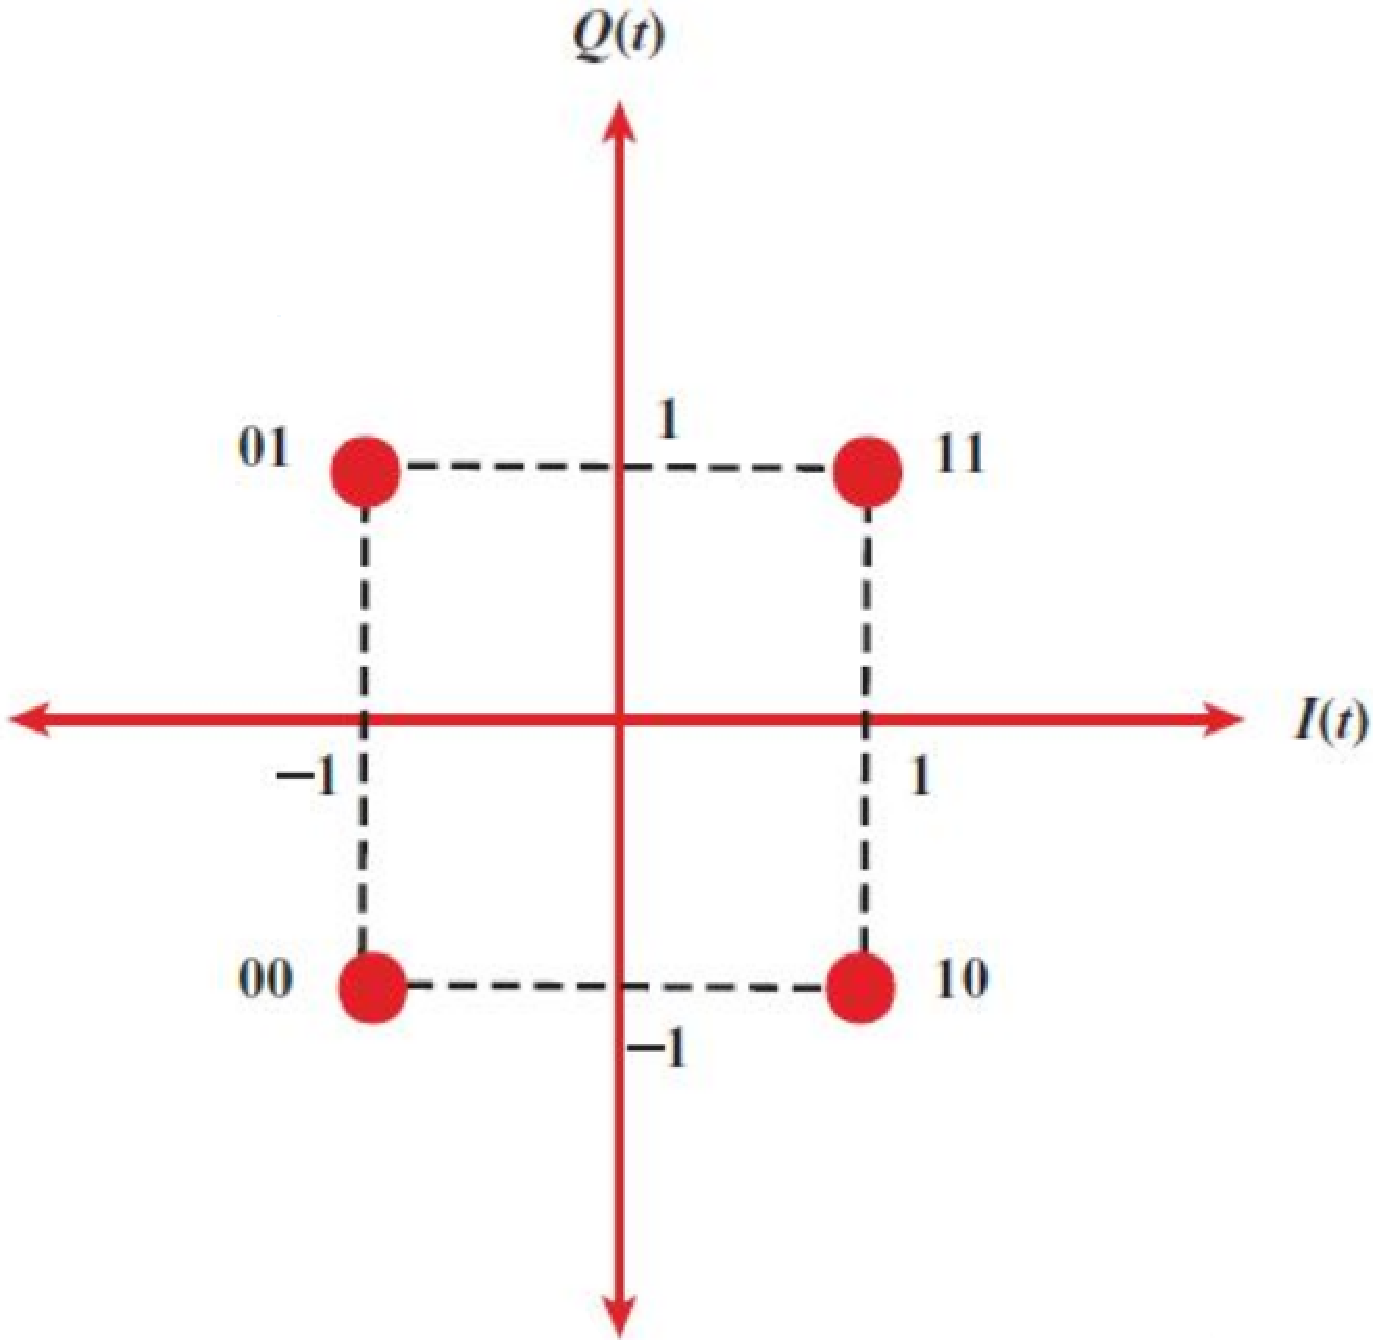
\includegraphics[width=0.45\linewidth]{img/wireless/costellazione1}
\end{center}
Si può vedere che ci sono 4 "posizioni", ognuna delle quali codifica 2 bit. Si chiama "quadra" per la variazione di $90^\circ$ tra uno e l'altro. Qua abbiamo 2 bit per symbol.\\

\newpage

\paragraph{Quadrature Amplitude Modulation QAM:} Oltre alla fase abbiamo anche una modifica dell'ampiezza. Utilizziamo due parametri per avere più codifiche differenti, portando ad una costellazione più densa. Combina variazioni di ampiezza e fase. 
\begin{center}
	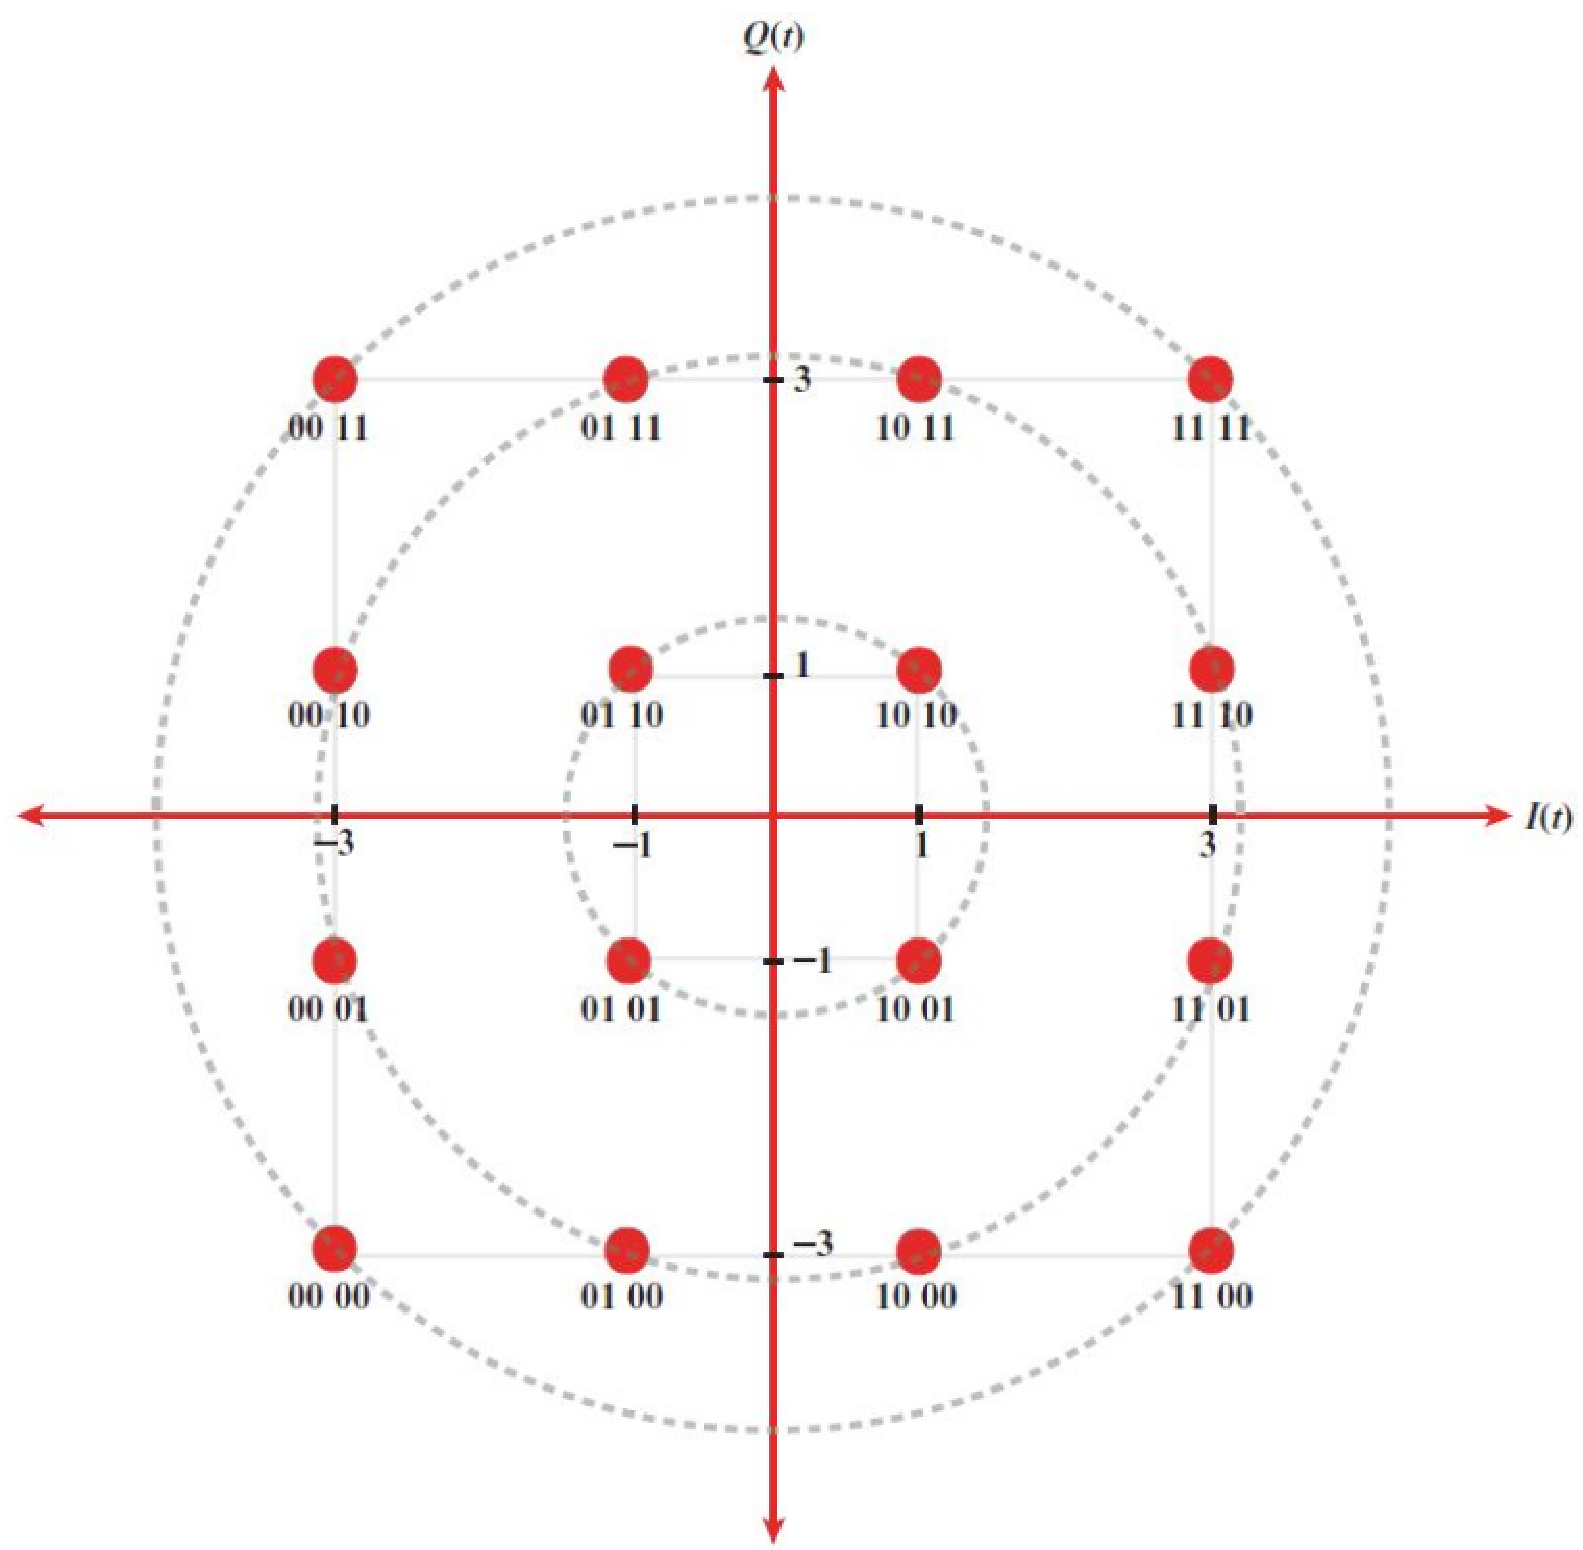
\includegraphics[width=0.6\linewidth]{img/wireless/costellazione2}
\end{center}
Schema QAM:
\begin{center}
	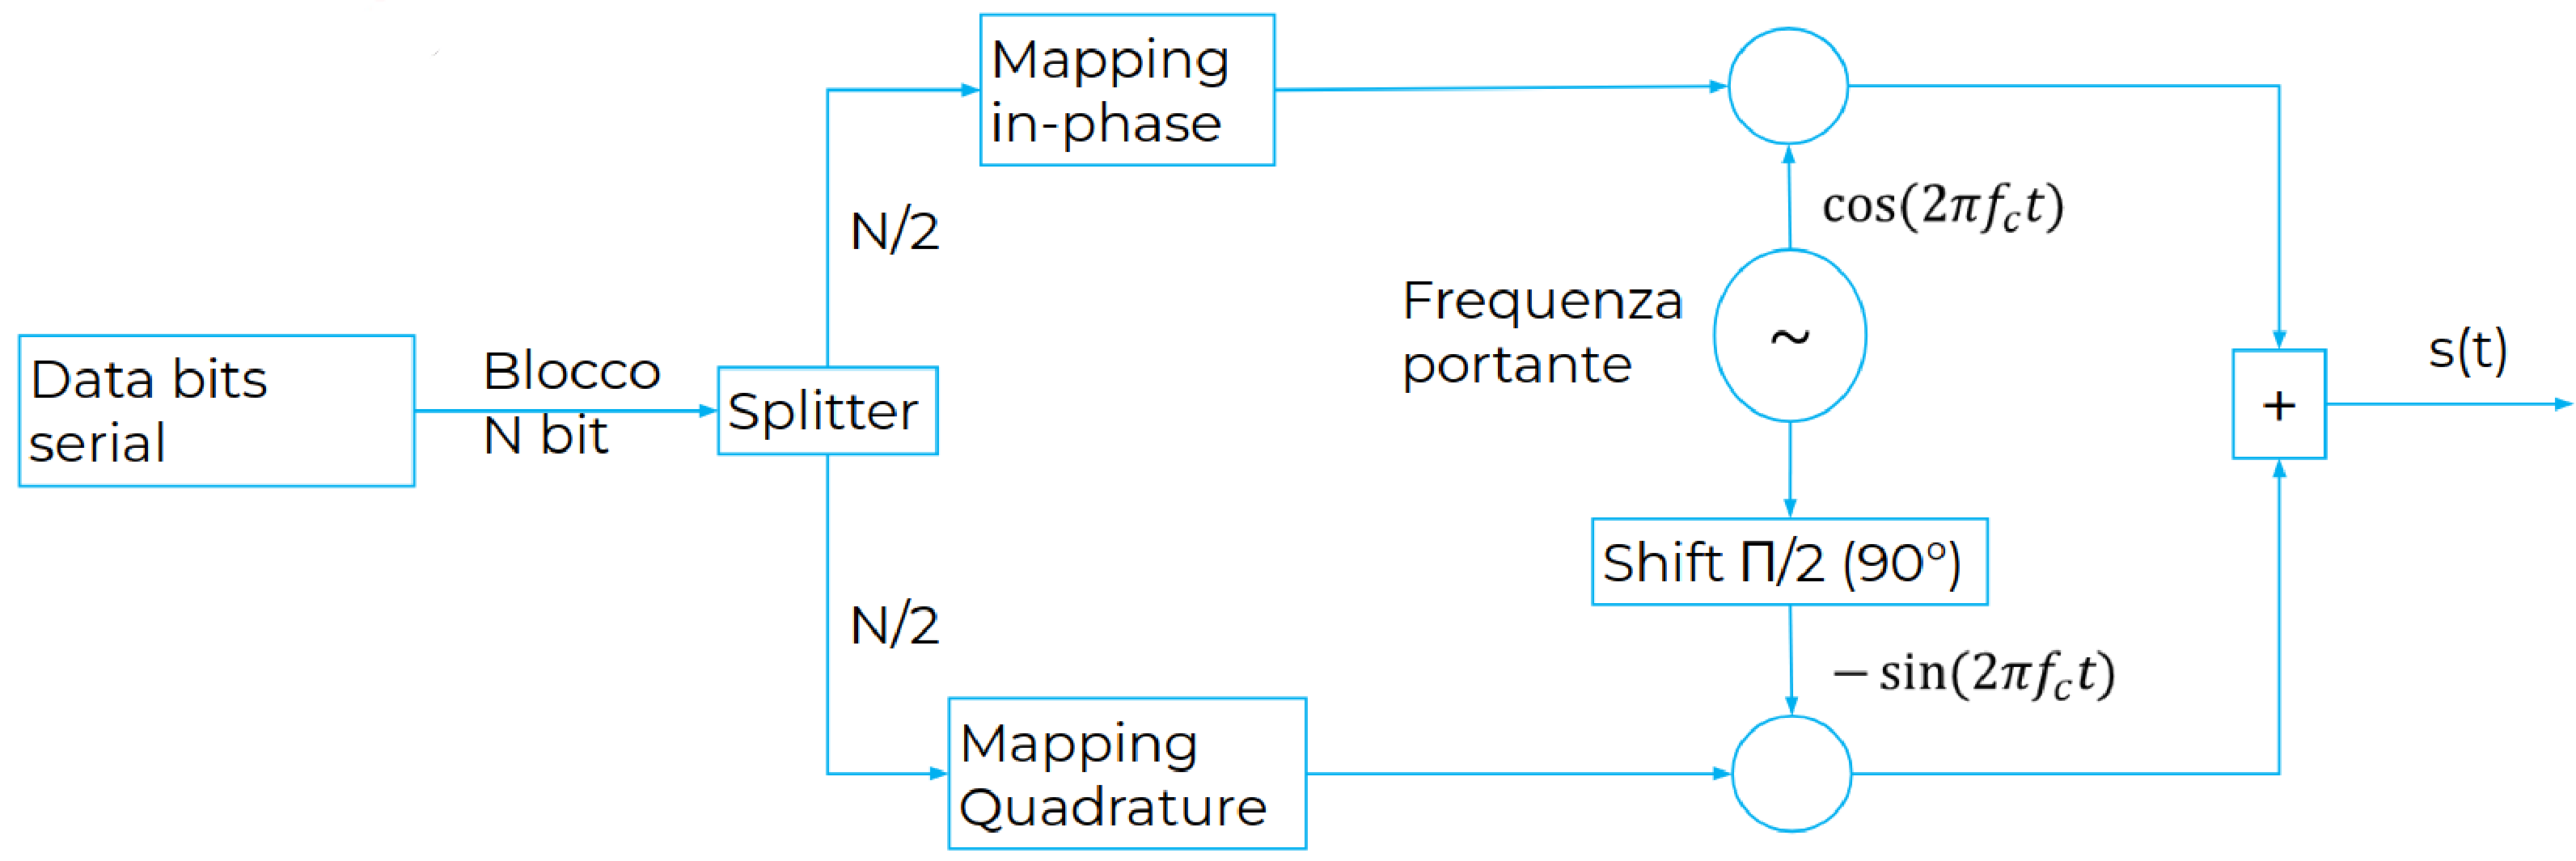
\includegraphics[width=0.9\linewidth]{img/wireless/schemaQAM}
\end{center}
Si spezzano i bit, si mappa prima in fase e poi in ampiezza, si modula sulla portante e le sinusoidi risultanti si uniscono per avere il segnale modulato da trasmettere.\\

%TODO: esempi slide 81,82, controllare, capire?
%Esempi maybe, idk anymore
% Esempi slides

Wi-Fi 5 usa 256-QAM mentre Wi-Fi 6 usa 1024-QAM. La potenza rimane costante, ci muoviamo all'interno dello stesso spazio, quello che cambia è quanto "densi" sono i simboli all'interno dello spazio.\\

\newpage

\subsubsection{Bit Error Rate Curve}
Rappresenta la \textbf{probabilità che un bit venga alterato}, in funzione del rapporto tra la densità di energia del segnale per bit ed il livello di rumore
$$ BER = func = \left( \frac{E_b}{N_0} \right)$$
Qual'è la probabilità di sbagliare un bit, dato un certo rapporto tra densità di energia del segnale per bit e rumore. Simile a SNR come idea.\\
Dei valori ricevuti da un trasmettitore potrebbero essere:
\begin{center}
	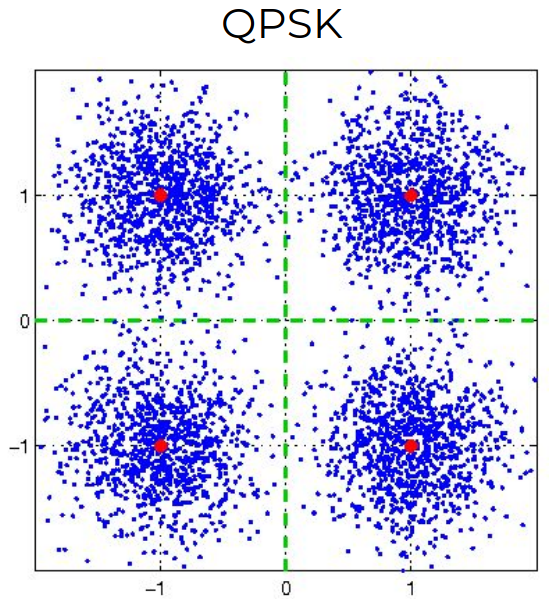
\includegraphics[width=0.35\linewidth]{img/wireless/esval}
\end{center}

Il RX riceve una "nuvola" di punti e cerca il simbolo più vicino ma se l'alterazione subita è significativa potrebbe essere un'interpretazione sbagliata quindi un errore. Man mano che il segnale migliora rispetto al rumore, la probabilità di avere un errore diminuisce. Tanto più densa è la costellazione tanto è più probabile sbagliare simbolo:
\begin{center}
	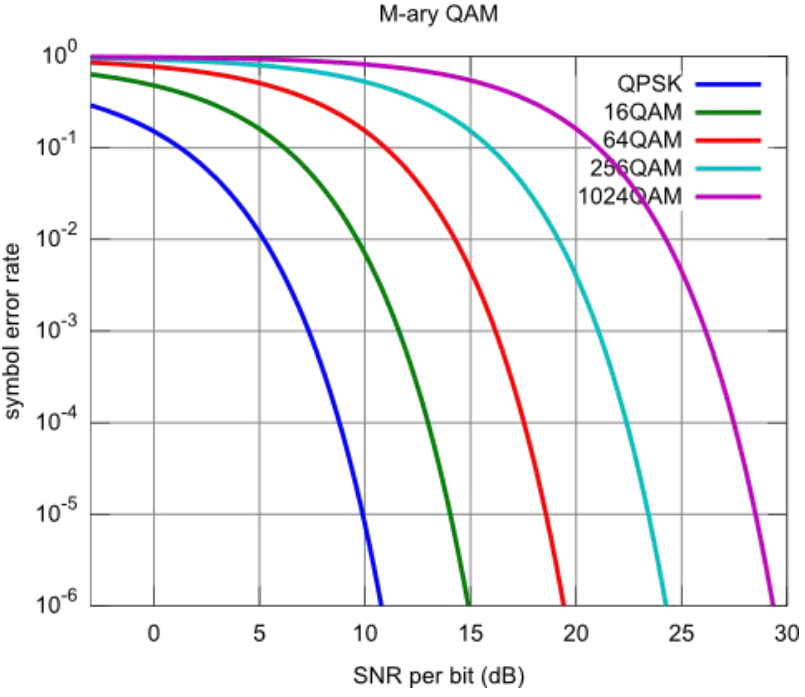
\includegraphics[width=0.5\linewidth]{img/wireless/maryqam}
\end{center}
Si può vedere come QPSK sbagli molto meno rispetto a 1024-QAM.

\newpage

\paragraph{Adaptive Modulation and Coding AMC:} Misuriamo la qualità del canale e cerchiamo di capire quale sia la codifica più efficiente, troppi errori renderebbero la comunicazione effettivamente inutile. Se il SNR è 10 è inutile trasmettere con 1024-QAM in quanto quasi tutti i simboli saranno sbagliati (immagine precedente), è meglio inviare con un data rate minore che permette meno errori. \\

La \textbf{codifica viene modificata in base alla qualità del canale}, ogni tot di tempo misuro la qualità del canale ed adatto il data rate di conseguenza.\\

\subsubsection{Forward Error Correction}
Servono delle tecniche di correzione dell'errore. Dato che nel wireless la probabilità di errore è elevata, viene aggiunta una ridondanza ai dati inviati: ogni sequenza di bit diventa una codeword, abbiamo $k$ bit trasmessi per $n$ bit da inviare (sempre $k>n$). In questo modo, con una tabella di codeword adatta, è possibile rendere la trasmissione resiliente agli errori.
\begin{center}
	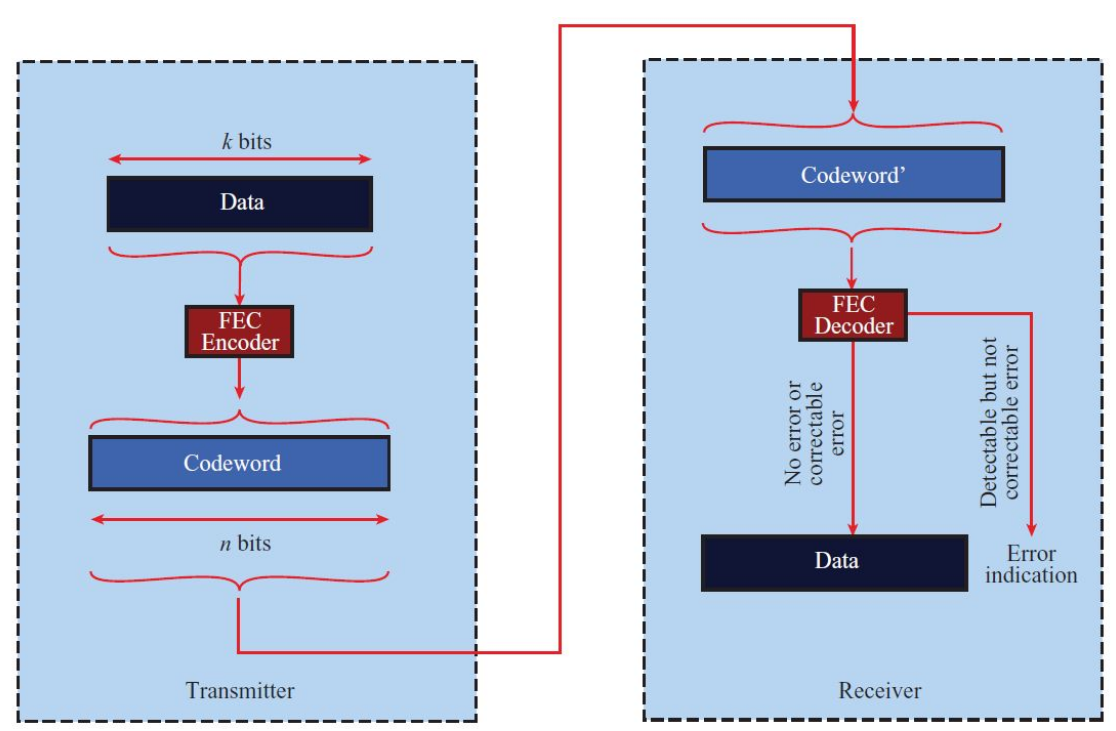
\includegraphics[width=0.7\linewidth]{img/wireless/FEC1}
\end{center}
Ogni $n$ bit da trasmettere diventano $k$, secondo una tabella prefissata, così anche se qualcuno arriva sbagliato si può ricostruire il valore originale (esempio: $00 \rightarrow 00000$, $10 \rightarrow 11001$).\\
Rimangono valide le tecniche di error detection, in cui a livello di RX riusciamo a capire se c'è stato un errore tramite dei bit di controllo aggiunti ai dati (e.g., CNC).\\

\paragraph{AMC:} A seconda delle condizioni del canale wireless il trasmittente sceglie lo schema di modulazione e codifica opportuno. Bisogna scegliere: codifica, coding rate (redundancy). Usato in nelle reti mobili 4G, 5G e WiFi (802.11n+).\\

Generalmente, queste informazioni vengono scelte a partire da una tabella: se ho un SNR di questo tipo, che modulazione e coding rate (rapporto bit totali e di informazione effettiva) posso usare?  
\begin{center}
	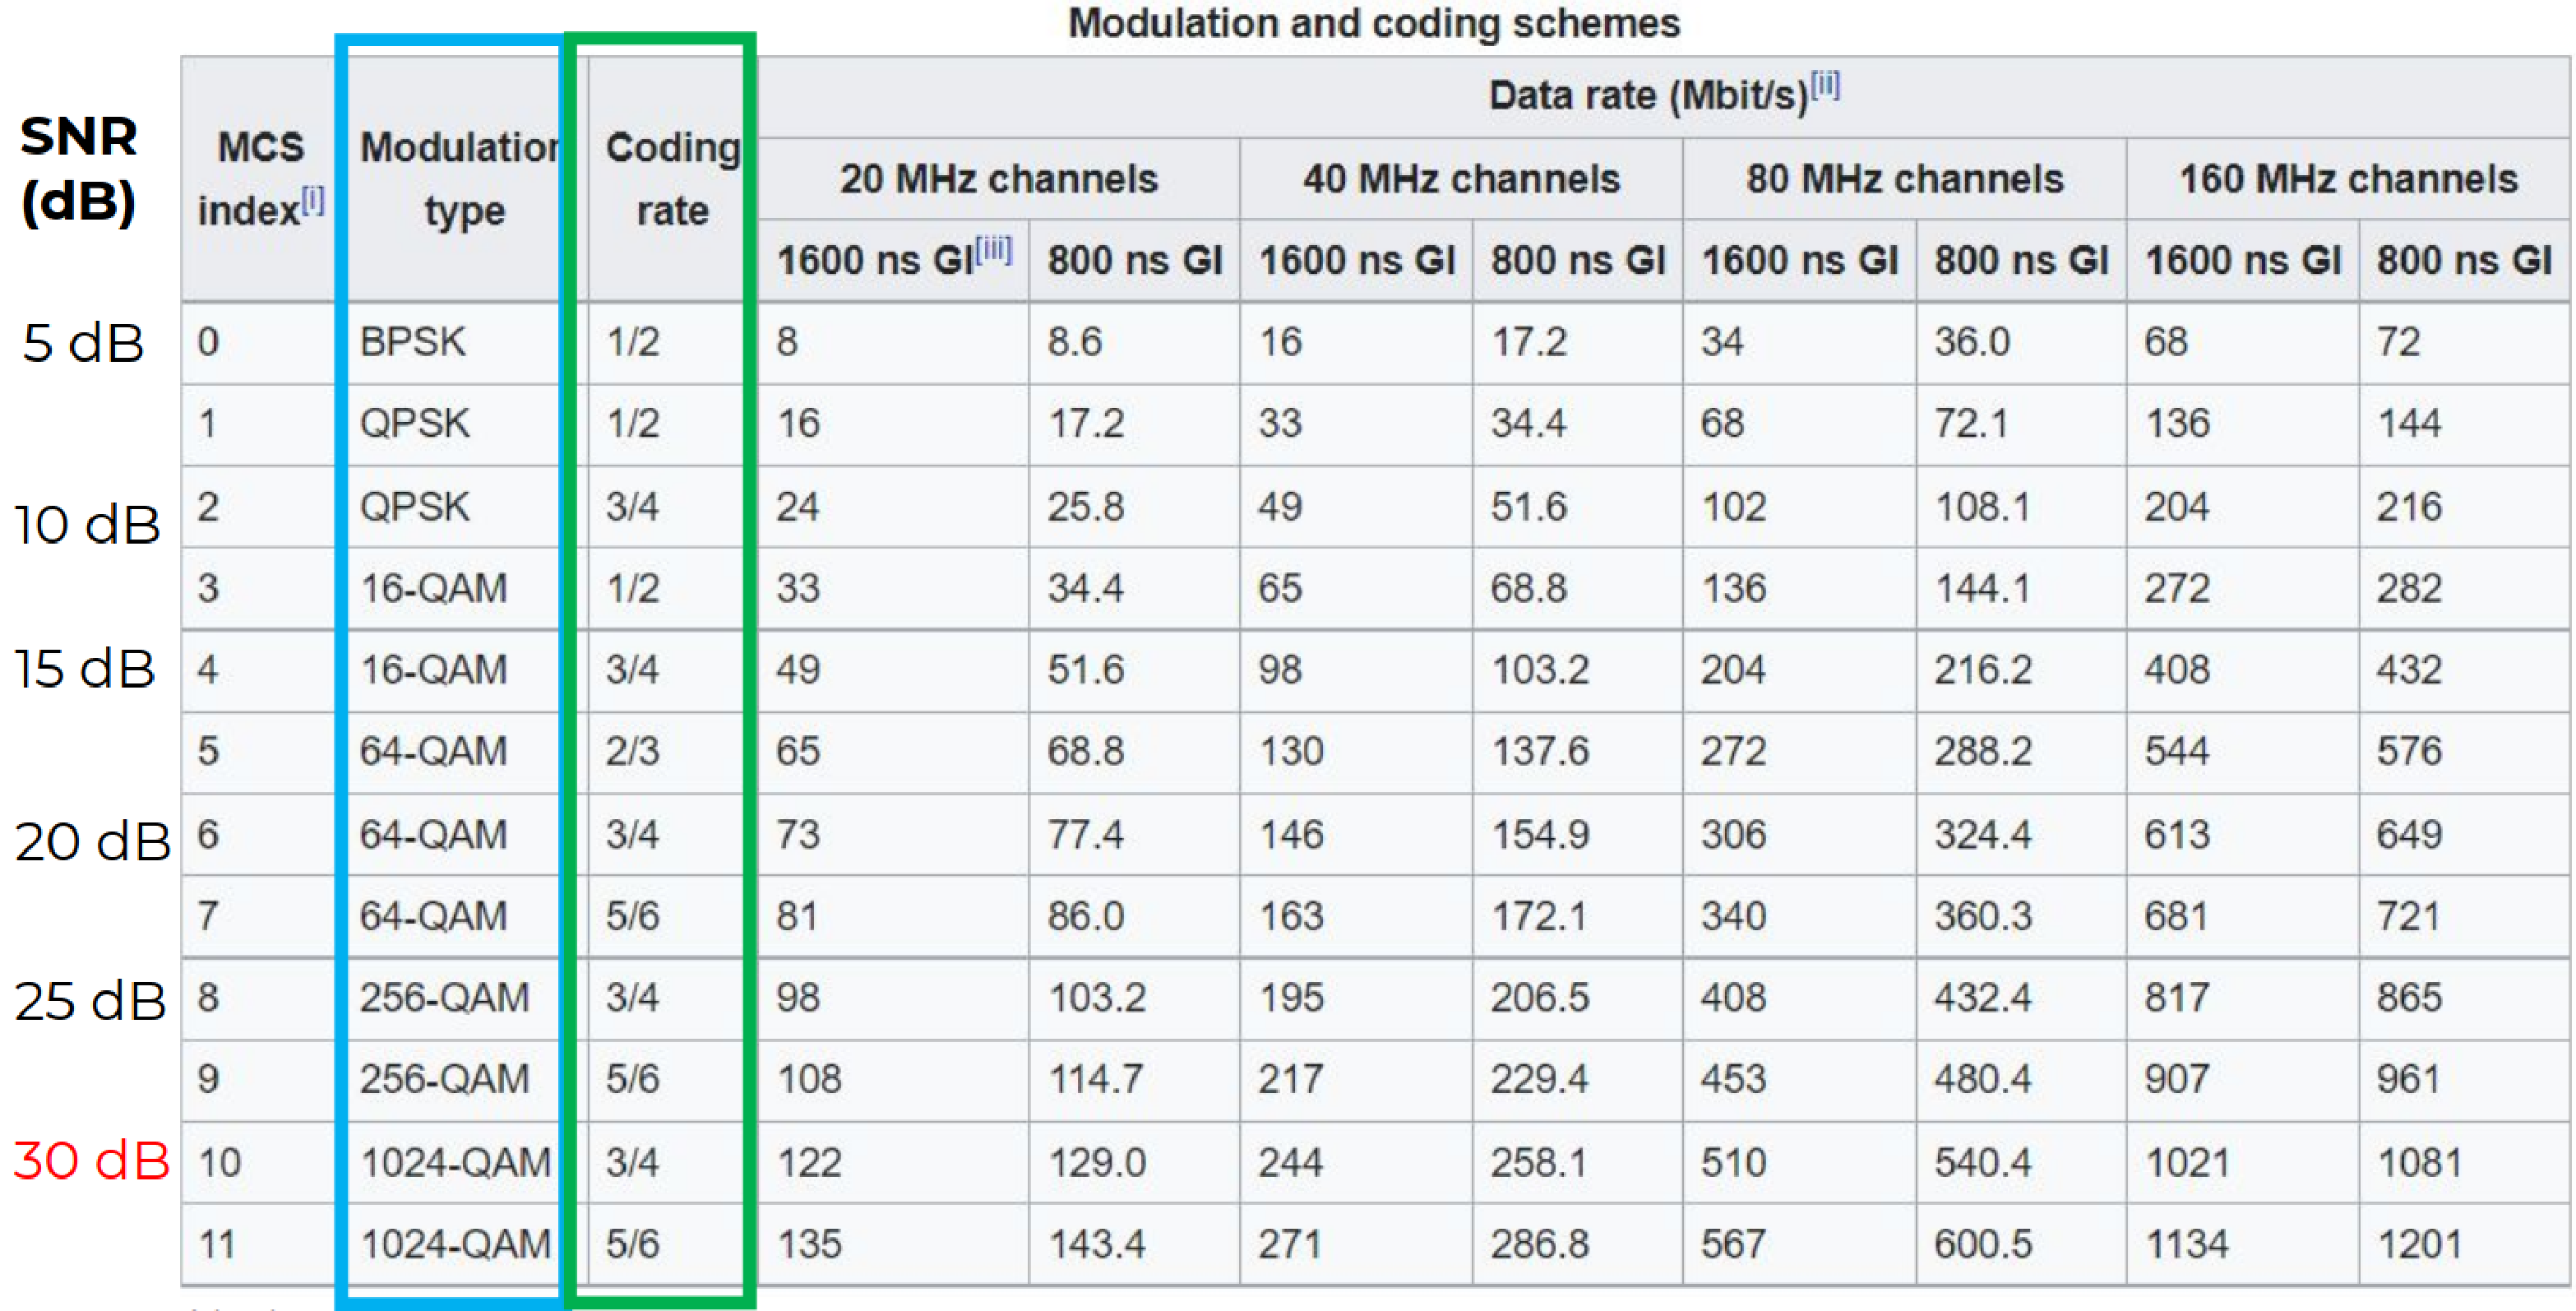
\includegraphics[width=0.95\linewidth]{img/wireless/mcruppolo}
\end{center}

%End L3

%start from s89
%Tipico esercizio d'esame su AMC
% Esercizio s89

\newpage

\paragraph{Esempio:} Dati un $SNR$ sul canale, un $BER$ che si vuole garantire ed un symbol rate
$$ SNR = 8dB, \; BER = 10^{-2}, \; SR = 1000 sym/s$$
Che modulation and coding scheme posso usare sul mio canale per avere l'error rate desiderato, sapendo che il coding rate per ogni codifica è
\begin{center}
	\begin{table}[h]
		\centering
		\begin{tabular}{|c|c|c|c|}
			\hline
			& \multicolumn{3}{c |}{\textbf{Coding rate}} \\
			\hline
			\textbf{SNR} & \textbf{BPSK} & \textbf{QPSK} & \textbf{16-QAM} \\
			\hline
			$< 6dB$ & 0.6 & 0.4 & 0.2 \\
			$6-10 dB$ & 0.8 & 0.6 & 0.5 \\
			$> 10 dB$ & 0.9 & 0.8 & 0.7 \\
			\hline
		\end{tabular}
	\end{table}
\end{center}
Ed il BER per ogni codifica è 
\begin{center}
		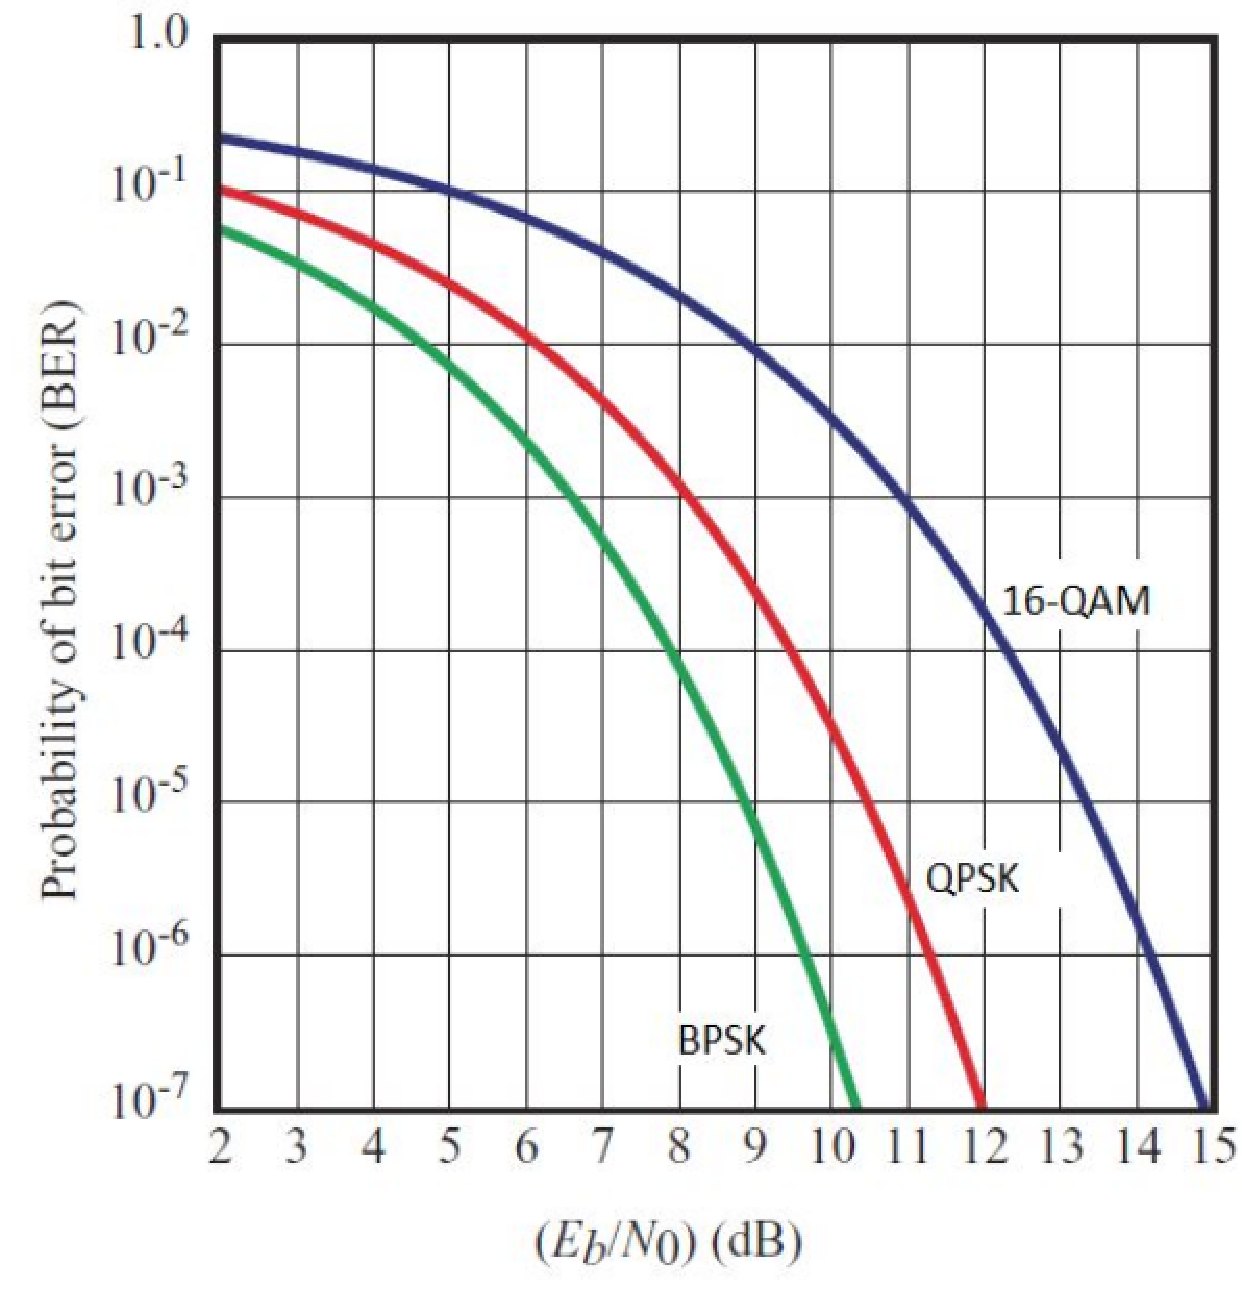
\includegraphics[width=0.45\linewidth]{img/wireless/esber}
\end{center}

Dall'immagine si può vedere che con $SNR = 8dB$, sia BPSK che QPSK permettono un $BER$ adeguato. Quale dei due però permette il data rate migliore? Possiamo calcolare il data rate come
$$ sym/s \cdot bit/sym \cdot coding\_rate $$
Quindi
\begin{itemize}
	\item BPSK: con coding rate di $0.8$ ed $1bps$: $1000 \cdot 1 \cdot 0.8 = 800 bit/s$
	\item QPSK: con coding rate di $0.6$ e $2bps$: $1000 \cdot 2 \cdot 0.6 = 1200 bit/s$
\end{itemize}

\newpage

\subsubsection{Orthogonal Frequency Division Multiplexing OFDM}
Vogliamo offrire canali differenti usando una divisione in frequenza diversa da FDM. L'obiettivo è quello di garantire lo stesso data rate che avremmo in una trasmissione in TDM ma usando una divisione in frequenza, senza usare troppa banda. Schema:
\begin{center}
	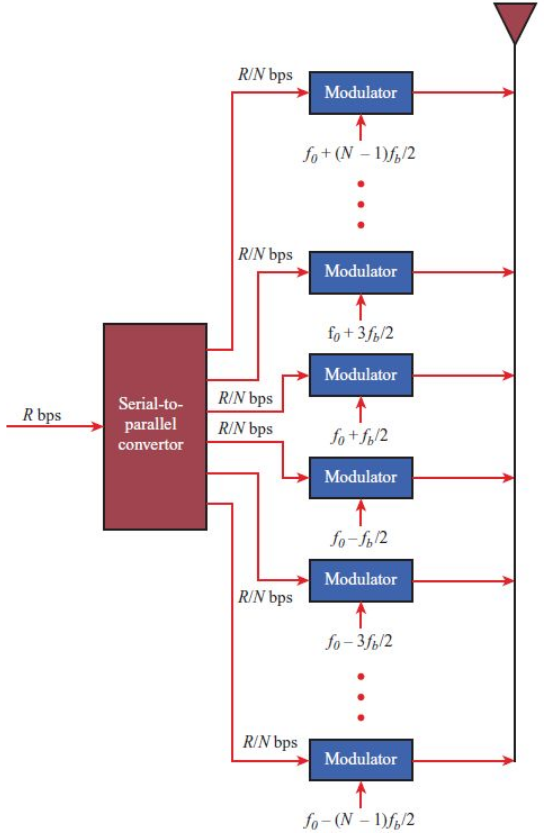
\includegraphics[width=0.45\linewidth]{img/wireless/OFDM1}
\end{center}
Lo si implementa tramite uno split da seriale a parallelo ed ogni componente viene inviata ad un modulatore, ognuno dei quali modula rispetto a multipli di una certa frequenza base $f_b$ e alla portante $f_0$; quindi abbiamo una portante $f_0$ e tante sotto-portanti multiple di $f_b$. Stessa codifica e modulazione. Alla fine si trasmette la combinazione di tutte le onde create. \\

Nel caso di FDM classico viene lasciata una guardia per evitare interferenze, si allontanano un po' le frequenze in modo tale che le varie armoniche di una frequenza non possa interagire con le adiacenti.\\

\newpage

\paragraph{Ortogonalità:} Nell'OFDM le \textbf{subcarrier sono ortogonali tra loro} e non interferiscono, i.e., la distanza tra subcarrier è studiata in modo da evitare interferenze. Nel momento di picco di ogni sotto-portante, il contributo delle altre frequenze è nullo.
\begin{center}
	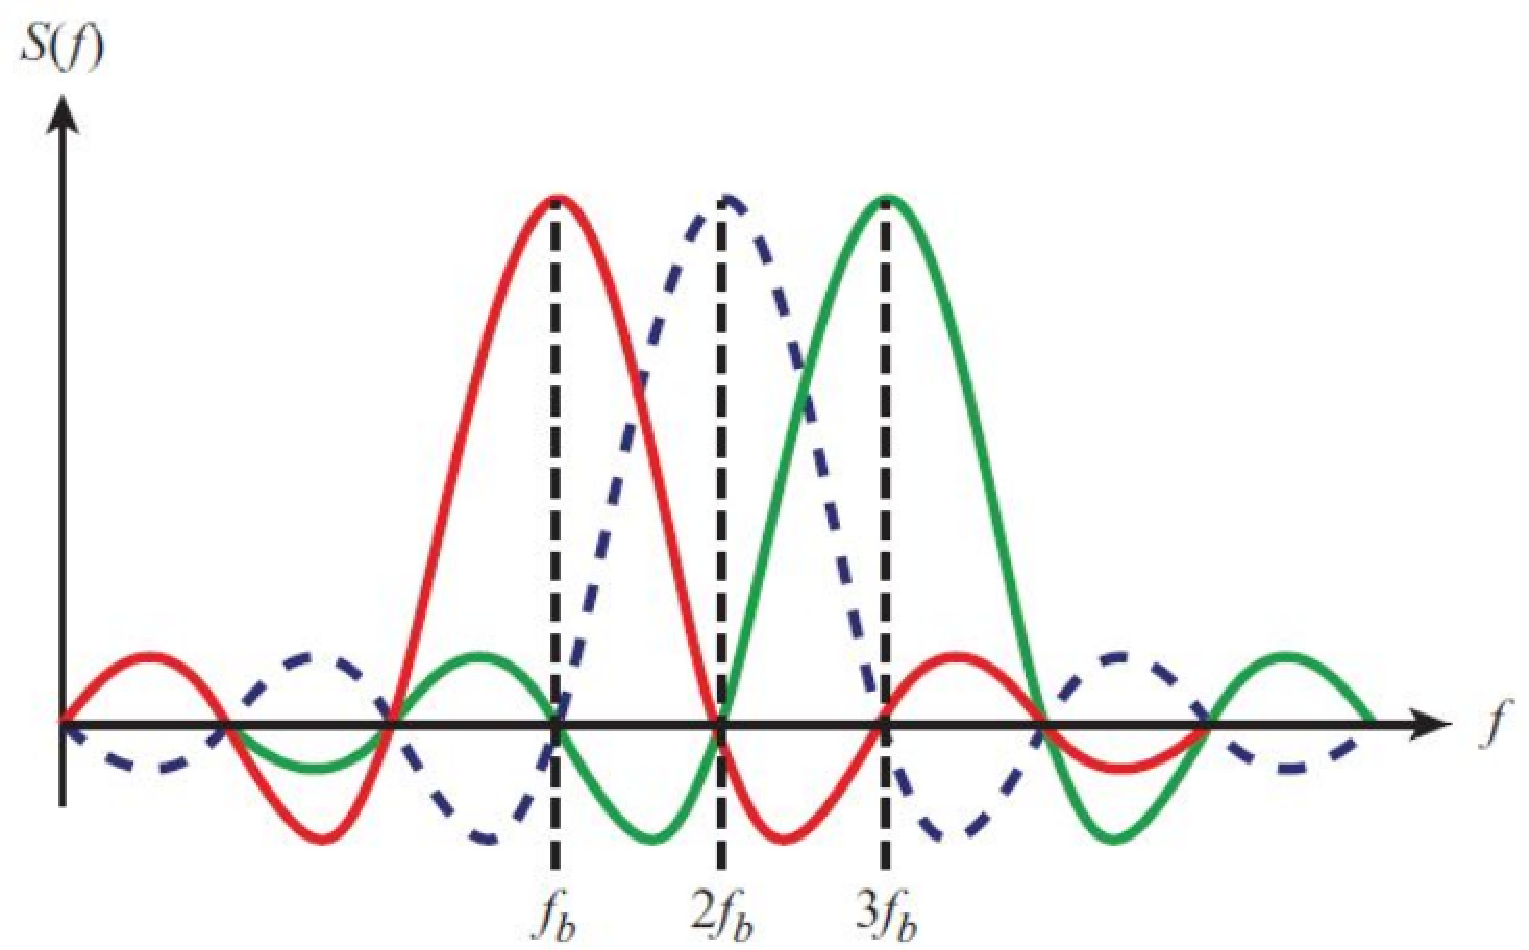
\includegraphics[width=0.6\linewidth]{img/wireless/OFDM2}
\end{center}

La scelta di $f_b$ dipende dalla durata dei simboli $T$:
$$ f_b = \frac{1}{T}$$
Tutti i segnali multipli di $f_b$ sono ortogonali tra loro. Si tratta dell'inverso della durata del simbolo.\\

Considerazioni:
\begin{itemize}
	\item più robusto riguardo ad interferenze che riguardano solo alcuni subcarrier
	\item più robusto rispetto ai problemi di multipath perché la distanza tra un simbolo e l'altro è maggiore (ISI ridotta)
\end{itemize}

N.B.: in generale multiple access $\neq$ multiplexing, far passare più segnali contemporaneamente è diverso da fare comunicare più utenti contemporaneamente.\\

\paragraph{TL;DR: } Si tratta di un FDM in cui le frequenze sono ortogonali tra loro in modo da non avere interferenze. Le interferenze in FDM erano prevenute tramite l'uso di una guardia, ovvero spazio di banda libero, OFDM permette di usare meno banda.\\

\newpage

\subsection{Spread Spectrum}
Letteralmente "spettro espanso", consiste nel trasmettere il segnale di informazione su uno \textbf{spettro di frequenze più ampio} di quella del segnale. Una banda maggiore del necessario. \\

La struttura, concettualmente, è
\begin{center}
	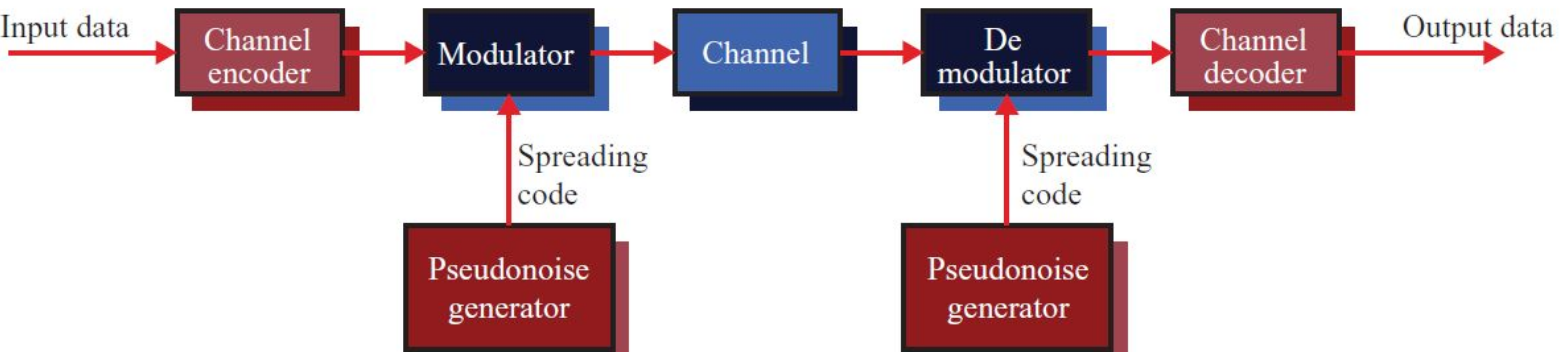
\includegraphics[width=0.95\linewidth]{img/wireless/ss1}
\end{center}
Dopo l'encoding, c'è una fase di \textbf{spreading dei dati}, generalmente basato su valori pseudo-casuali (da invertire dopo la ricezione).\\

Motivazioni:
\begin{itemize}
	\item rendere il segnale più robusto, "spalmandolo" su una banda più ampia lo rende più resiliente a diversi tipi di rumore e interferenze
	\item nascondere e cifrare il segnale (nato in ambito militare); solo TX e RX sono a conoscenza del codice di spreading (non una tecnica sufficiente, ma a livello radio questo si può fare)
	\item molti utenti possono usare indipendentemente la stessa banda contemporaneamente senza interferenza. Usata da CDMA
\end{itemize}

\newpage

\subsubsection{Frequency Hopping Spread Spectrum FHSS}

In FHSS il codice di spreading determina quale frequenza usare per trasmettere il segnale. Ad ogni intervallo di tempo prestabilito, la frequenza viene cambiata pseudo-casualmente (frequency hopping). usato da Bluetooth (802.15.1), "saltando" ogni $625 \mu s$.\\
In altre parole: ho una certa ampiezza di banda e cambio in modo pseudo-casuale la frequenza usata ad ogni intervallo di tempo. Ho $n$ frequenze e ne uso una per volta, cambiata ogni tanto.\\

Schema di trasmissione e ricezione:
\begin{center}
	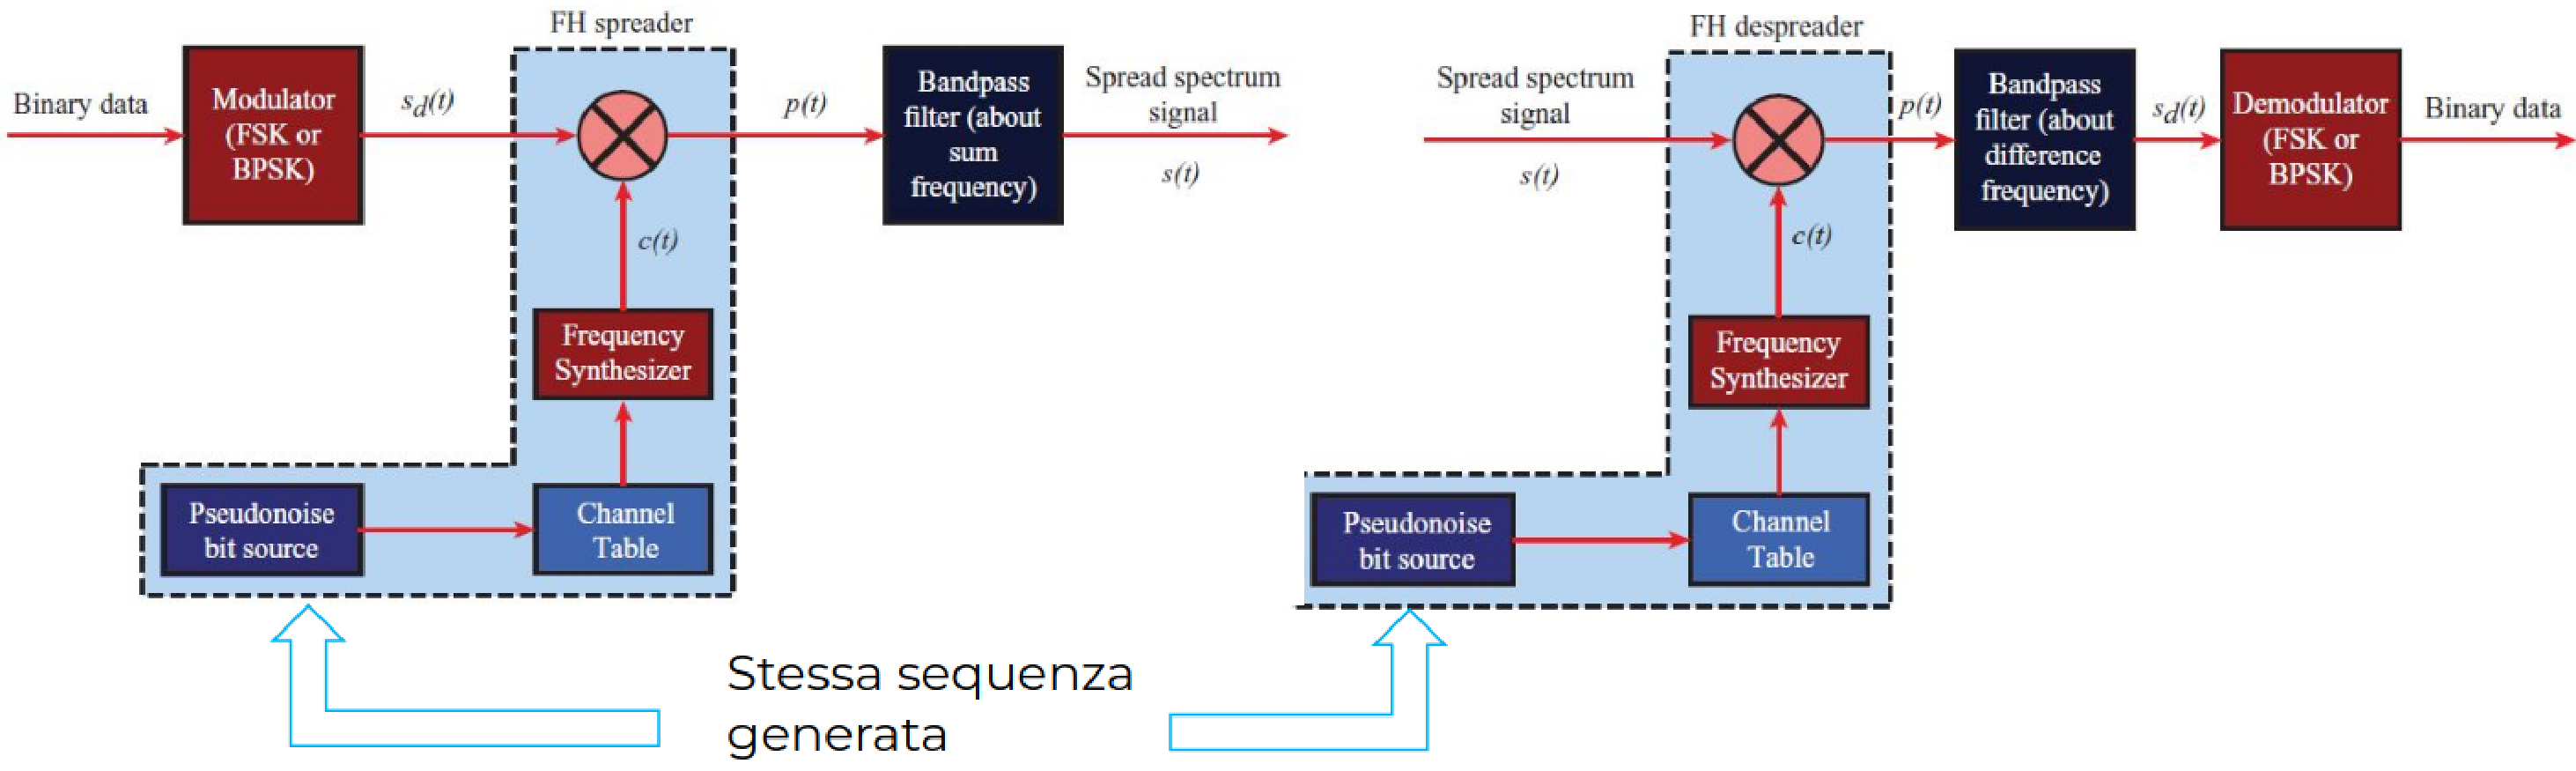
\includegraphics[width=\linewidth]{img/wireless/fhss1}
\end{center}
La channel table permette di scegliere la frequenza da utilizzare, in base al valore casuale, ed il sintetizzatore utilizzerà quella frequenza. Il tempo di hopping generalmente è predefinito, serve un seed per la sequenza di valori pseudo-casuali usati per determinare la frequenza usata.\\

Il frequency hopping è più resistente a rumore e jamming, in quanto compromettere una frequenza non compromette l'intera trasmissione.\\
Un altro ricevitore che si sincronizza con il trasmettitore può solo leggere alcuni pezzi dei messaggi perché non conosce la sequenza di hopping. \\

\newpage

\subsubsection{Direct Sequence Spread Spectrum DSSS}

Per una sequenza di $D$ bit, ogni bit della sequenza viene rappresentato da un insieme di bit usando un codice di spread (pseudo-casuale). Ogni bit diventa $n$ bit ottenuti da una sequenza casuale. \\
I bit della sequenza di spread "durano meno" (durano $1/n$ del tempo dei bit di informazione) e vengono chiamati "chip". Per ogni bit originale abbiamo $n$ chip.\\
Per mantenere lo stesso data rate abbiamo bisogno di $n$ volte la banda ($n$ fattore di spreading).\\

Generalmente, si usa uno \texttt{xor} (in quanto invertibile) degli $n$ bit casuali con il bit da inviare e si invia il risultato. Esempio: 
\begin{center}
	\begin{tabular}{|c|c|c|c|c|c|c|c|c|}
		\hline
		\multicolumn{1}{|c|}{\textbf{Bit informazione}} & \multicolumn{4}{c|}{\textbf{1}} & \multicolumn{4}{c|}{\textbf{0}} \\ 
		\hline
		\textbf{Sequenza di chip} & 0 & 1 & 1 & 1 & 0 & 0 & 1 & 0 \\ 
		\hline
		\textbf{Trasmesso (XOR)} & 1 & 0 & 0 & 0 & 0 & 0 & 1 & 0\\ 
		\hline
	\end{tabular}
\end{center}
Usando BPSK diventa: 
\begin{center}
	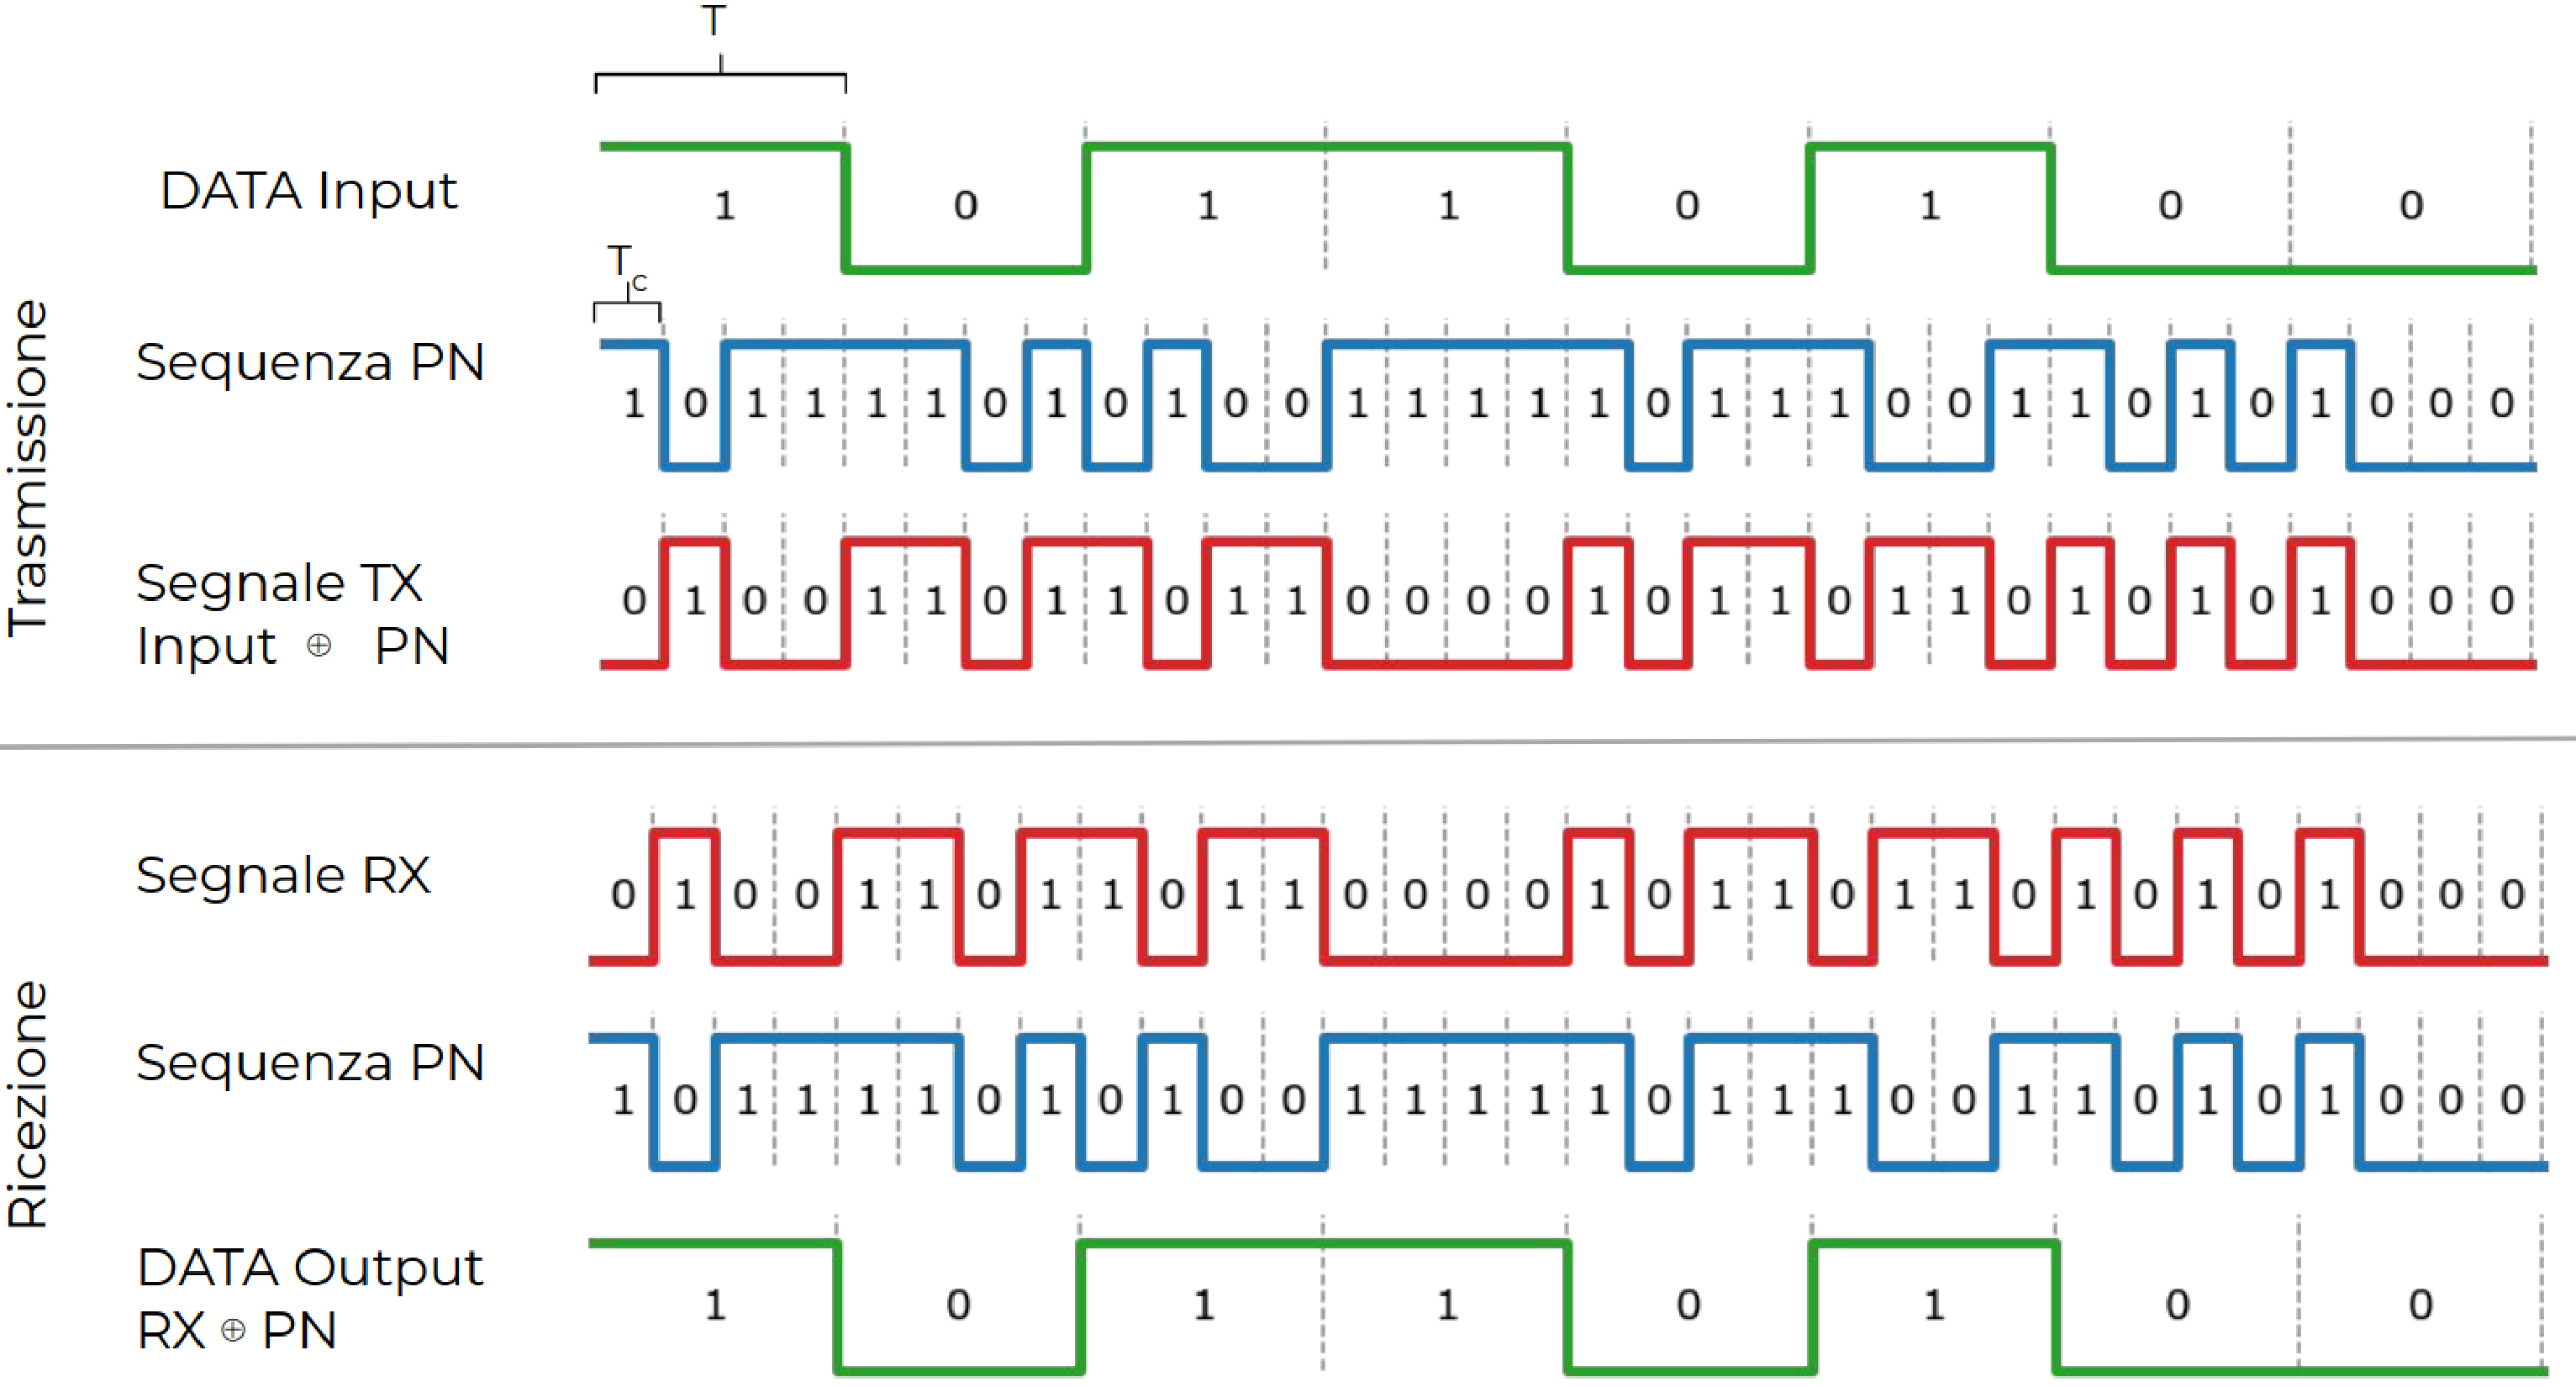
\includegraphics[width=0.95\linewidth]{img/wireless/DSSS1}
\end{center}
In verde il {\color{green} segnale originale}, in blu la {\color{blue} sequenza pseudo-casuale}, in rosso ciò che viene {\color{red} effettivamente inviato}.\\

%Schema di trasmissione e ricezione: 
%img s110

%End L4